%% 
%% Copyright 2019-2020 Elsevier Ltd
%% 
%% This file is part of the 'CAS Bundle'.
%% --------------------------------------
%% 
%% It may be distributed under the conditions of the LaTeX Project Public
%% License, either version 1.2 of this license or (at your option) any
%% later version. The latest version of this license is in
%%    http://www.latex-project.org/lppl.txt
%% and version 1.2 or later is part of all distributions of LaTeX
%% version 1999/12/01 or later.
%% 
%% The list of all files belonging to the 'CAS Bundle' is
%% given in the file `manifest.txt'.
%% 
%% Template article for cas-dc documentclass for 
%% double column output.

\documentclass[conference]{IEEEtran}

% IEEE Access packages
\usepackage{cite}
\usepackage{amsmath,amssymb,amsfonts}
\usepackage{algorithmic}
\usepackage{graphicx}
\usepackage{textcomp}
\usepackage{xcolor}

% \usepackage[authoryear,longnamesfirst]{natbib}
%\usepackage[authoryear]{natbib}
\usepackage[numbers,sort&compress]{natbib}

\usepackage{algorithm}
\usepackage{algpseudocode}
\renewcommand{\algorithmicrequire}{\textbf{Input:}}  % Use Input in the format of Algorithm  
\renewcommand{\algorithmicensure}{\textbf{Output:}} % Use Output in the format of Algorithm 

\usepackage{threeparttable}%表格下面加标注
\usepackage{rotating}

% Attempt to fix the \pdf@box issue: load graphicx with pdftex driver and color
%\usepackage[pdftex]{graphicx}
%\usepackage{color}

% Now load hyperref (also with pdftex driver to be consistent? Actually, hyperref will use the driver automatically)
%\usepackage{hyperref}
\usepackage{float}
\usepackage{array, longtable, tabularx}
%\usepackage{caption}

\usepackage{cleveref} % 确保 cleveref 已加载
\crefname{figure}{}{}% 设置 \cref 对 figure 的引用格式为空(只留编号)
\Crefname{figure}{}{}% 设置 \Cref 对 figure 的引用格式为空(只留编号)
\crefname{table}{}{}% 设置 \cref 对 figure 的引用格式为空(只留编号)
\Crefname{table}{}{}% 设置 \Cref 对 figure 的引用格式为空(只留编号)
\crefname{section}{}{}% 设置 \cref 对 figure 的引用格式为空(只留编号)
\Crefname{section}{}{}% 设置 \Cref 对 figure 的引用格式为空(只留编号)
\usepackage{float}
\usepackage{array, longtable, tabularx}

\sloppy
%%%Author definitions
\def\tsc#1{\csdef{#1}{\textsc{\lowercase{#1}}\xspace}}
\tsc{WGM}
\tsc{QE}
\tsc{EP}
\tsc{PMS}
\tsc{BEC}
\tsc{DE}
%%% 

\begin{document}
\let\ref\Cref 		
\let\eqref\Cref 	
\let\autoref\Cref 	
\let\WriteBookmarks\relax
\def\floatpagepagefraction{1}
\def\textpagefraction{.001}
\shorttitle{Journal of Engineering Research xx (20xx) xxxxxx}
\shortauthors{Author 1 and N.S. Ahmad}
\footmarks{\url{https://doi.org/10.1016/j.jer.20xx.xx.xxx}\\
    0952-1976/\begingroup\tiny{©}\endgroup~2025 Elsevier B.V.\\
    This is an open access article under the CC BY-NC-ND license (\url{http://creativecommons.org/licenses/by-nc-nd/4.0/}).
}


% \bookmark[named = FirstPage]{A Comprehensive Survey on UWB-Based NLOS Identification and Ranging Error Mitigation Using CIR Features and Raw Sequences} % Title bookmark used in the pdf
%**************** If the title is short, stay on the first line use [mode = short_title] otherwise ******************
%***************************************** use [mode = title] below ***************************************
\title{Perception-to-Action Benchmarks for Autonomous Fruit-Picking Robots: Quantitative Synthesis, Gaps, and Deployment Roadmap}

% Title mark notes if desired
%\tnotemark[1,2]

%\tnotetext[1]{This document is the results of the research
%   project funded by the National Science Foundation.}

%\tnotetext[2]{The second title footnote which is a longer text matter
%   to fill through the whole text width and overflow into
%   another line in the footnotes area of the first page.}

\author{\IEEEauthorblockN{Zhihao Zhao}
\IEEEauthorblockA{\textit{School of Electrical and Electronic Engineering} \\
\textit{Universiti Sains Malaysia}\\
Nibong Tebal, Malaysia \\
email@usm.my}
\and
\IEEEauthorblockN{Nur Syazreen Ahmad}
\IEEEauthorblockA{\textit{School of Electrical and Electronic Engineering} \\
\textit{Universiti Sains Malaysia}\\
Nibong Tebal, Malaysia \\
syazreen@usm.my}}

\credit{Conceptualization of this study, Methodology}

\address[1]{School of Electrical and Electronic Engineering, Universiti Sains Malaysia, 14300 Nibong Tebal, Penang, Malaysia}

\author[3]{Yanxiang Zhao}
\author[1]{Nur Syazreen Ahmad}[type=author, 
                        auid=001,bioid=2,
                        orcid=0000-0001-7511-2910
                        ]
%\fnmark[1]
\cormark[1]
% \ead{syazreen@usm.my}
\credit{Data curation, Writing-Original draft preparation}

\address[2]{YanTai Engineering and Technology College, 264006 YanTai, Shandong, China}
\address[3]{Central South University, Changsha, Hunan, 410083, China}
% \author[1,3]{CV Radhakrishnan}[type=editor, 
%                         auid=000,bioid=1,
%                         prefix=Sir,
%                         %role=Researcher,
%                         %orcid=0000-0001-7511-2910
%                         ]
% \cormark[1]
% %\fnmark[1]								% URL related footnote marking
% \ead{cvr_1@tug.org.in}
% %\ead[url]{www.cvr.cc, cvr@sayahna.org} % Author URL 

% \credit{Conceptualization of this study, Methodology, Software}

% \address[1]{Elsevier B.V., Radarweg 29, 1043 NX Amsterdam, The Netherlands}

% \author[2,3]{Han Theh Thanh}[style=chinese]

% \author[2,3]{CV Rajagopal}[
%    %role=Co-ordinator,
%    suffix=Jr,
%    ]
% %\fnmark[2]								% URL related footnote marking
% \ead{cvr3@sayahna.org}
% %\ead[URL]{www.sayahna.org}				% Author URL

% \credit{Data curation, Writing - Original draft preparation}

% \address[2]{Sayahna Foundation, Jagathy, Trivandrum 695014, India}

% \author
% [1,3]
% {Rishi T.} % If the author's name hits "Check for updates" button, use \\ at the break point of his/her name like {\\Rishi T.} or {First Middle\\ Lastname}
% % NOTE: Compile first without \\ then the proper separation again afterwards !!! (Not doing so, results unwanted footnote and Credit authorship contribution at the very end with \credit command if used.)
% \cormark[2]
% %\fnmark[1,3]							% URL related footnote marking
% \ead{rishi@stmdocs.in}
% %\ead[URL]{www.stmdocs.in}				% Author URL

% \address[3]{STM Document Engineering Pvt Ltd., Mepukada,
%     Malayinkil, Trivandrum 695571, India}

% \author[4]{ \\Salih Baris Ozturk} % Author's name hits "Check for updates" button, \\ is used at the break point of his name. If \\ is desired at the beginning of the name, place a space just before the \\ as in the above example.
% % NOTE: Compile first without \\ and the space, then the proper separation again afterwards !!! (Not doing so, results unwanted footnote and Credit authorship contribution at the very end with \credit command if used.)
% %\cormark[1]
% \ead{ozturksb@itu.edu.tr}

% \address[4]{Istanbul Technical University, Department of Electrical Engineering,
% 	Maslak, Istanbul 34469, Turkey}

\credit{Modification for the final layout}

\cortext[1]{Corresponding author.}
% \cortext[cor2]{Principal corresponding author.}
% \fntext[1]{E-mail address: \href{mailto:syazreen@usm.my}{syazreen@usm.my} (N.S. Ahmad).}
%\fntext[fn2]{Another author footnote, this is a very long footnote and
%  it should be a really long footnote. But this footnote is not yet
%  sufficiently long enough to make two lines of footnote text.}

%\nonumnote{This note has no numbers. In this work we demonstrate $a_b$
%  the formation Y\_1 of a new type of polariton on the interface
%  between a cuprous oxide slab and a polystyrene micro-sphere placed
%  on the slab. The evanescent field of the resonant whispering 
%  gallery mode (\WGM) of the micro sphere has a substantial 
%  gradient, and therefore effectively couples with the
%  quadrupole $1S$ excitons in cuprous oxide.}

\nonumnote{E-mail address: \href{mailto:syazreen@usm.my}{syazreen@usm.my} (N.S. Ahmad).}

\begin{abstract} 
This review synthesizes recent advances in autonomous fruit-picking robots with a focus on visual perception, path planning, and motion control. Following PRISMA guidelines, we systematically analyzed 137 studies published between 2015 and 2024. We critically compare learning-based perception approaches—especially YOLO- and R-CNN–family methods—under orchard-specific conditions (occlusion, variable lighting, small targets), and quantify trade-offs in accuracy and efficiency across representative platforms. We further examine perception-to-action integration for motion planning and control, summarizing success rate, harvest cycle time, and damage rate reported in field and greenhouse trials. 

Learning-based approaches, including transfer learning and reinforcement learning (e.g., Deep Deterministic Policy Gradient), have enhanced the generalizability of robotic arm motion planning for collision-free harvesting. Innovative path-planning algorithms and robust control strategies enable autonomous robots to navigate unstructured environments and compensate for real-time disturbances, increasing system reliability. Despite these advances, persistent challenges remain in multi-source data integration, delicate fruit handling, and cost-effective scalability. This survey provides a comprehensive evaluation of technological progress, identifies critical research gaps in deployment and scalability, and proposes future directions to accelerate commercial adoption in diverse agricultural contexts.
\end{abstract}

% If any graphical abstract is needed
%\begin{graphicalabstract}
%\includegraphics{figs/grabs.pdf}
%\end{graphicalabstract}

% If any highlights is needed above the cover page
%\begin{highlights}
%\item Research highlights item 1
%\item Research highlights item 2
%\item Research highlights item 3
%\end{highlights}

% Article history - Should only be set by an editor
\received {xx Month 20xx}
\revised {xx Month 20xx}
\accepted {xx Month 20xx}
\online {xx Month 20xx}

\begin{keywords}
 Autonomous Fruit-Picking Robots,
Regions with Convolutional Neural Networks (R-CNN),
You Only Look Once (YOLO),
Motion Planning,
Transfer Learning.
\end{keywords}

\maketitle

\section{Introduction}
Farms worldwide are grappling with labor shortages, skyrocketing costs, and demands for sustainable methods. Autonomous fruit-picking robots offer a promising answer, drawing on AI, vision tech, and robotics that could streamline harvests while ease worker burdens. Just how close are we to robots that rival human pickers? This review dives in. 
%Autonomous fruit-picking robots are revolutionizing agriculture by tackling labor shortages, rising costs, and the push for greater harvesting efficiency. These systems draw on cutting-edge tools like computer vision, machine learning (ML), robotics, and Internet of Things (IoT) to navigate varied farm settings, gently handle produce, and support human workers. 

Recent breakthroughs in machine learning (ML), deep learning (DL) and sensor fusion have enhanced robots' capacity to discern, localize, and manipulate objects with greater precision. These developments have been reviewed and summarized in Table ~\ref{tab:survey_summary}. They have also addressed deficiencies in end-to-end integration.
%The advent of autonomous fruit-picking robots signifies a substantial advancement in agricultural technology, precipitated by the necessity to address labor shortages, escalating costs, and the demand for enhanced efficiency in fruit production.
%Rapid advancements in robotics and artificial intelligence have catalyzed substantial interest in developing fruit-picking robots. These robots promise to revolutionize agricultural practices by automating labor-intensive fruit harvesting. Fruit-picking robots are autonomous systems engineered to identify, locate, and harvest fruits from various trees and plants. 
%These systems leverage advanced technologies, including computer vision, machine learning (ML), robotics, and the Internet of Things (IoT), to operate efficiently in diverse agricultural environments, handle fruits delicately, and complement human labor.
%These systems leverage a suite of advanced technologies, including computer vision, machine learning (ML), robotics, and Internet of Things (IoT). The aim is to create robots that can operate efficiently in various agricultural environments, handle fruits delicately to avoid damage, and work alongside human labor to enhance productivity. 
%like Figure~\ref{fig:fruit_picking_robot_overview}.
%Recent advancements in deep learning (DL) and sensor fusion have facilitated the development of sophisticated perception and motion control mechanisms, enabling robots to detect, localize, and harvest fruits with increasing precision.
 Figure ~\ref{fig:struct} illustrates the general architecture of an autonomous fruit-picking robot, highlighting key components such as visual sensors for detection, manipulator arms for grasping, and navigation systems for mobility. This advancement has been particularly evident in addressing challenges such as occlusion, variable lighting, and unstructured orchards.

Existing literature reviews have laid the groundwork for understanding strides in autonomous fruit-picking technologies as summarized in Table~\ref{tab:survey_summary}. These recent surveys, all published since 2021, have collectively advanced the field by addressing various aspects of robotic systems, though they often exhibit limitations in scope and integration.
For instance, Hou et al. \cite{hou2023overview} focused on the integration of deep learning (DL) with multi-sensor vision systems, emphasizing perception sensors and machine vision to enhance fruit detection in unstructured environments. While this work provided valuable insights into AI-driven fusion and trends in field robustness, it overlooked broader system integration and actuation mechanisms. Similarly, Navas et al. \cite{navas2021soft} specialized in soft and bionic gripper designs, advancing understanding of adaptive handling for delicate fruits from a mechanical perspective, but neglected upstream components like perception or downstream integration, resulting in a siloed approach.
In contrast, more comprehensive reviews such as those by Zhang et al. \cite{zhang2024automatic} and Mingyou et al. \cite{mingyou2024orchard} adopted end-to-end perspectives. Zhang et al. covered machine vision, motion planning, end-effectors, mechanical automation, system integration, and field adaptation, notably including real-time control via IoT/5G and economic feasibility assessments for practical deployment. Mingyou et al. extended this by addressing multi-robot coordination and large-scale perception in expansive orchard settings, innovating with robust mapping and cooperative robotics trends. These works excelled in promoting holistic views but were sometimes constrained by their emphasis on specific deployment scenarios, such as large-scale orchards, potentially limiting applicability to smaller or diverse crop types.
Other surveys, including Zhou et al. \cite{zhou2022intelligent} and Rajendran et al. \cite{rajendran2024towards}, emphasized modular architectures and precision control. Zhou et al. explored machine vision, motion planning, and field adaptation, highlighting vision-driven precision and scalable designs for orchard autonomy, though without delving into mechanical details or cooperative elements. Rajendran et al. integrated perception sensors, machine vision, end-effectors, and field adaptation to discuss dexterous control and selective harvesting synergies, improving real-field reliability, yet their scope was somewhat narrow, focusing on targeted operations without broader multi-crop generalizations. Collectively, these surveys advanced the field by identifying key performance indicators, such as detection accuracy and adaptability metrics, but their fragmentation—often isolating components like perception from action or constraining to specific fruits (e.g., apples or citrus)—left gaps in fully end-to-end frameworks that encompass diverse agricultural contexts.
%This section reviews the primary contributions of some key surveys, highlighting their scopes and insights, followed by a discussion of their collective limitations, which motivate the innovations in this paper.
%Hou et al. \cite{hou2023overview}  focused on the integration of deep learning (DL) with multi-sensor vision systems. Their survey emphasized perception sensors and machine vision, detailing how AI-driven fusion enhances fruit detection in unstructured environments. This work highlighted trends in field robustness but overlooked broader system integration and actuation mechanisms.
%Zhang et al. \cite{zhang2024automatic}  provided an end-to-end perspective on automation chains, covering machine vision, motion planning, end-effectors, mechanical automation, system integration, and field adaptation. A notable contribution was the inclusion of real-time control via IoT/5G and economic feasibility assessments, offering a holistic view of practical deployment.
%Navas et al. \cite{navas2021soft} specialized in soft and bionic gripper designs, concentrating exclusively on end-effectors. Their analysis advanced understanding of adaptive handling for delicate fruits, drawing from mechanical perspectives, though it neglected upstream components like perception or downstream integration.
%Zhou et al. \cite{zhou2022intelligent} explored modular architectures, with emphasis on machine vision, motion planning, and field adaptation. Key insights included vision-driven precision and robot autonomy in orchards, promoting scalable designs that enhance adaptability without delving into mechanical details or cooperative elements.
%Mingyou et al. \cite{mingyou2024orchard}  addressed multi-robot coordination and large-scale perception, covering machine vision, motion planning, mechanical automation, system integration, and field adaptation. This survey innovated by focusing on robust mapping and execution in expansive orchard settings, incorporating cooperative robotics trends.
%Rajendran et al. \cite{rajendran2024towards} integrated perception sensors, machine vision, end-effectors, and field adaptation to discuss precision and dexterous control. Their contribution centered on selective harvesting synergies, improving real-field reliability for targeted operations.

%While these surveys collectively advance the discourse on fruit-picking robotics, several limitations persist that hinder a fully integrated and forward-looking understanding of the field. First, many exhibit a narrow temporal scope or outdated coverage; 
%While prior surveys have advanced the field as summarized in Table ~\ref{tab:survey_summary}, they exhibit limitations that our work addresses. 
%For instance, many have a narrow temporal scope, focusing predominantly on literature before 2020 and overlooking recent breakthroughs in DL models like YOLOv8.
% Zhou et al. and Navas et al. end in 2021, missing pivotal post-2022 developments in AI and multimodal sensing. Hou et al. and Rajendran et al. extend to 2022-2023 but underexplore emerging trends like unified benchmarking or cost-feasibility analyses, which are critical for industrial translation.
%A deeper issue is the siloed focus on specific subsystems: Navas et al. isolates end-effectors without linking to perception-action loops, while Hou et al. prioritizes vision but ignores motion planning and mechanical automation. This fragmentation leads to incomplete end-to-end frameworks, as seen in the absence of system integration in several works (e.g., Hou, Navas, Zhou, and Rajendran). Moreover, cooperative robotics and benchmarking are inconsistently addressed. Mingyou et al. touches on multi-robot aspects, but others largely omit them, resulting in a lack of standardized evaluation metrics for cross-study comparisons. Zhang et al. makes strides in economic feasibility, yet this is not uniformly integrated across surveys, often overlooking practical barriers like deployment costs and scalability in diverse agricultural contexts.
% Additionally, several adopt a siloed approach, emphasizing isolated aspects such as detection or grasping without integrating them into a cohesive end-to-end framework. This fragmentation underscores gaps in holistic analyses, which we bridge through a 'perception-action' approach that encompasses multi-sensor fusion, visual perception, and motion control.
%These limitations collectively underscore a gap in synthesizing multimodal fusion, perception-action integration, and roadmap-oriented guidance for future research. Without addressing these, the field risks redundant efforts and delayed real-world adoption.

The survey under discussion addresses the limitations of prior works, including fragmented subsystem analyses, insufficient end-to-end integration, and the absence of unified benchmarking and scalability considerations. It does so by introducing a holistic "perception-action" framework.
We critically evaluate technological breakthroughs, identify persistent challenges, and propose future directions to accelerate commercial adoption.
%Drawing from the foundational insights of surveys like Hou et al. on deep learning fusion, Zhang et al. on complete automation chains, and Mingyou et al. on multi-robot coordination, this paper emphasizes synergistic integrations that bridge gaps in real-world applicability. 
%Specifically, it focuses on: (1) multi-modal sensor fusion (integrating IoT, remote sensing, and vision \cite{mohamed2021smart,martos2021ensuring,liu2024hierarchical}) with advanced DL models (e.g., evolved YOLO architectures) to overcome detection fragility in dynamic environments, extending beyond the vision-centric approaches in Hou et al. and Rajendran et al.; (2) linking visual perception outputs (e.g., fruit stem localization \cite{li2023mta}) with adaptive path planning (e.g., LiDAR-fused trajectory optimization \cite{liu2024hierarchical}) for seamless operations in unstructured terrain, addressing siloed motion planning in Zhou et al. and Mingyou et al.; and (3) incorporating collaborative robotics principles \cite{lytridis2021overview,li2023multi} alongside system-level efficiency and cost-feasibility analyses to tackle scalability challenges overlooked in component-focused reviews like Navas et al.

The core contributions of this survey are thus:
\begin{itemize}
\item A systematic analysis of multi-modal strategies aligned with DL models to enhance detection robustness in diverse agricultural scenarios.
% bridging fragmented discussions.
% in prior surveys.

\item A comprehensive quantitative comparison of fruit detection models, evaluating trade-offs in accuracy 
 and efficiency 
 %(e.g., 5 ms-0.467 s per image)
, coupled with a dissection of core metrics (reliability, precision, rapidity) from last decade, including strengths 
%(e.g., 96\% tomato detection, 28 ms apple inference) 
and limitations 
%(e.g., 5.27\% occluded citrus error)
, to provide decision frameworks and interconnections for holistic optimization.
% extending metrics absent in prior works .
%like Rajendran et al.

\item An integrated synthesis of robotic motion control systems and perception-to-action pipelines for fruit harvesting, spanning diverse fruits and strategies from multi-DOF manipulators to visual servoing, quantifying variances 
%(e.g., 18-84\% success rates, 4-24 s cycle times) 
and interconnections with environmental factors
% overcoming narrow scopes for real deployment.
%in Zhou et al. and Navas et al.

\item A critical evaluation of collaborative robotic systems, unifying multi-arm coordination with cost-effective designs and benchmarking.
% to address scalability barriers underexplored in prior reviews.
% like Mingyou et al. and Zhang et al.
\end{itemize}

\begin{figure}[h!]
    \centering
    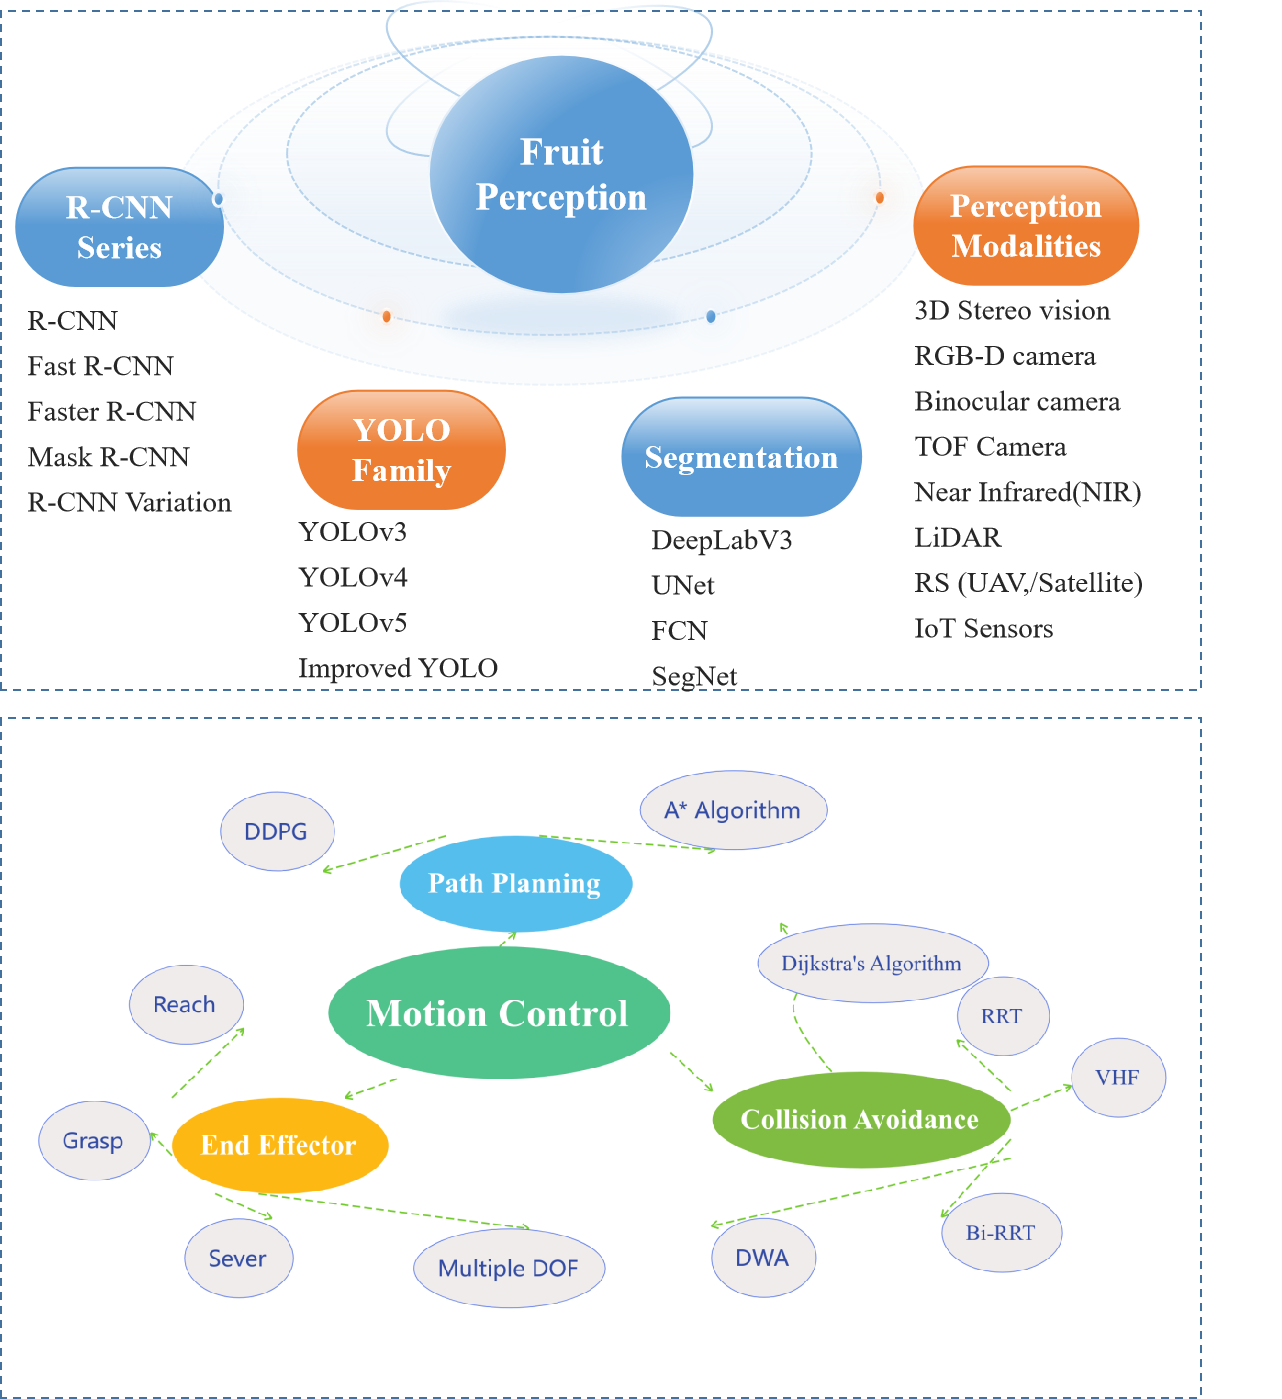
\includegraphics[width=0.55\textwidth]{fig_struct2.png}
    \caption{The perception-action framework of autonomous Fruit-Picking robots.}
    \label{fig:struct}
\end{figure}

\begin{table*}[htbp]
\centering
\footnotesize
\caption{Expanded Review Scope and Core Contributions of Major Fruit-Picking Robot Survey Papers}
\renewcommand{\arraystretch}{1.2}
\begin{tabular}{
    p{0.03\textwidth}  % Ref.
    p{0.075\textwidth}  % Year Range
    *{7}{>{\centering\arraybackslash}p{0.07\textwidth}} % Focus Scope x7
    p{0.22\textwidth}   % Summary
}
\hline
\multirow{2}{*}{\textbf{Ref.}}
& \multirow{2}{*}{\textbf{Range}}
& \multicolumn{7}{c}{\textbf{Focus Scope}}
& \multirow{2}{*}{\textbf{Trends}} \\
\cline{3-9}
&& \footnotesize Percep. Sensors
& \footnotesize Machine Vision
& \footnotesize Motion Planning
& \footnotesize End-Effectors
& \footnotesize Mechanical Automation
& \footnotesize System Integration
& \footnotesize Field Adaptation
& \\
\hline
\cite{hou2023overview}      & 2001-2022
& \ensuremath{\checkmark} & \ensuremath{\checkmark} & \ensuremath{\times} & \ensuremath{\times} & \ensuremath{\times} & \ensuremath{\times} & \ensuremath{\times}
& Deep learning fusion \\

\cite{zhang2024automatic}   & 1968-2023
& \ensuremath{\times} & \ensuremath{\checkmark} & \ensuremath{\checkmark} & \ensuremath{\checkmark} & \ensuremath{\checkmark} & \ensuremath{\checkmark} & \ensuremath{\checkmark}
& End-to-end automation \\

\cite{navas2021soft}        & 1993-2021
& \ensuremath{\times} & \ensuremath{\times} & \ensuremath{\times} & \ensuremath{\checkmark} & \ensuremath{\times} & \ensuremath{\times} & \ensuremath{\times}
& Soft gripping advances \\

\cite{zhou2022intelligent}  & 2012-2021
& \ensuremath{\times} & \ensuremath{\checkmark} & \ensuremath{\checkmark} & \ensuremath{\times} & \ensuremath{\times} & \ensuremath{\times} & \ensuremath{\checkmark}
& Modular architecture \\

\cite{mingyou2024orchard}   & 2003-2023
& \ensuremath{\times} & \ensuremath{\checkmark} & \ensuremath{\checkmark} & \ensuremath{\times} & \ensuremath{\checkmark} & \ensuremath{\checkmark} & \ensuremath{\checkmark}
& Multi-robot perception \\

\cite{rajendran2024towards} & 1995-2022
& \ensuremath{\checkmark} & \ensuremath{\checkmark} & \ensuremath{\times} & \ensuremath{\checkmark} & \ensuremath{\times} & \ensuremath{\times} & \ensuremath{\checkmark}
& Precision harvesting \\
This work & 2015-2024
& \ensuremath{\checkmark} & \ensuremath{\checkmark} & \ensuremath{\checkmark} & \ensuremath{\checkmark} & \ensuremath{\checkmark} & \ensuremath{\checkmark} & \ensuremath{\checkmark}
& Perception-action integration, \newline Multimodal integration \\
\hline
\end{tabular}
\label{tab:survey_summary}
\end{table*}

\iffalse
Existing reviews summarized in Table~\ref{tab:survey_summary} have laid valuable groundwork in autonomous fruit-picking robotics, however, they predominantly focus on fragmented components: individual sensor deployments (e.g., IoT or remote sensing in isolation \cite{mohamed2021smart,martos2021ensuring}), standalone model advancements (e.g., MTA-YOLACT for segmentation \cite{li2023mta}), or single-algorithm path planning (e.g., hierarchical trajectory methods \cite{liu2024hierarchical}). 
%While these works have advanced understanding of multi-sensor fusion, DL-based detection, and motion control techniques, 
They lack a critical systems-level perspective—failing to address how these components interact as an integrated ecosystem.
Notably, prior reviews overlook three pivotal gaps: (1) they rarely explore how multi-sensor fusion (e.g., LiDAR-vision integration \cite{liu2024hierarchical}) can be strategically paired with DL models to enhance robustness against real-world variability like occlusion or lighting changes; (2) they insufficiently connect visual perception (e.g., ripeness detection \cite{hou2023overview}) to context-aware motion planning tailored for unstructured orchards; and (3) they neglect the end-to-end optimization of collaborative systems (e.g., multi-arm coordination \cite{li2023multi}) that bridge perception, planning, and actuation.

This survey addresses these limitations by adopting a holistic "perception-action" framework. It uniquely emphasizes the synergistic integration of: (1) multi-modality sensor fusion (combining IoT, remote sensing, and vision \cite{mohamed2021smart,martos2021ensuring,liu2024hierarchical}) with DL models (e.g., evolved YOLO architectures) to mitigate detection fragility in dynamic environments; (2) visual perception outputs (e.g., fruit stem localization \cite{li2023mta}) with adaptive path planning (e.g., LiDAR-fused trajectory optimization \cite{liu2024hierarchical}) for seamless operation in unstructured terrain; and (3) collaborative robotics principles \cite{lytridis2021overview,li2023multi} with system-level efficiency analysis to address scalability challenges.


The core contributions of this survey are thus:
\begin{itemize}
\item A systematic analysis of how multi-sensor fusion strategies can be optimally aligned with DL models to enhance detection robustness across diverse agricultural scenarios, filling the gap in fragmented sensor-model discussions.
\item  A comprehensive quantitative analysis on fruit detection models, systematically comparing architectural trade-offs in accuracy (e.g., 87.83\%-99.5\% AP and efficiency (e.g., 5 ms-0.467 s per image) across diverse agricultural scenarios, and establishing decision frameworks for model selection based on specific orchard characteristics (such as greenhouse/outdoor environments, fruit density, and lighting conditions).
\item A systematic dissection of three core performance metrics (reliability, precision, rapidity) in fruit detection over the past decade, quantifying their strengths (e.g., 96\% detection rate for ripe tomatoes via color-based methods, 28 ms/image inference speed for apples) and limitations (e.g., 5.27\% relative error in occluded citrus contour analysis, speed-accuracy trade-off in small fruit detection), while establishing interconnections between metrics to guide holistic performance optimization in agricultural robotics.
\item A comprehensive synthesis of robotic motion control systems for fruit harvesting , spanning diverse fruits (apple, sweet pepper, strawberry, etc.) and control strategies (multi-DOF manipulators, dual-arm coordination, visual servoing), which quantifies performance gaps (e.g., 18-84\% success rate variance, 4-24 s cycle time range) and identifies critical interconnections between motion planning algorithms, environmental complexity, and harvesting efficiency to guide robotic system optimization in unstructured agricultural settings.
%\item An integrated exploration of perception-to-action pipelines, connecting visual insights to motion planning algorithms specifically tailored for orchard complexity.
%\item A critical evaluation of collaborative robotic systems that unify multi-arm coordination with cost-effective design principles, addressing scalability barriers overlooked in prior component-focused reviews.
\end{itemize}
\fi

The main structure of this paper is outlined in Figure \ref{fig:struct}; accordingly, the remainder of the review is organized as follows. Section II describes the overall methodology, including the search strategy, paper selection, and synthesis of findings. Section III provides a synthesis and comparative discussion of data acquisition approaches through multi-sensor fusion.
%analysis of existing fruit-picking methodologies, focusing on emerging challenges, the evolution of AI vision methods, and strategies to overcome limitations in detection and motion planning. 
Section IV discusses advances in visual perception for fruit-picking robotics, covering state-of-the-art vision models (including R-CNN, YOLO, and segmentation), and core performances metrics of fruit-picking robotics. Section V reviews advances and trends in motion control for robotic fruit harvesting, emphasizing algorithmic path planning, obstacle avoidance, and developments in motion planning and control. Section VI presents recent progress and future directions in autonomous fruit harvesting technologies. Finally, Section VII concludes the paper, summarizing key findings and outlining prospects for future research.



\section{Survey Methodology}
This survey follows the Preferred Reporting Items for Systematic Reviews and Meta-Analyses (PRISMA) guidelines \cite{page2021prisma} for a systematic and transparent process-key to avoiding bias in a field evolving this fast. 

\begin{figure}[h!]
    \centering
    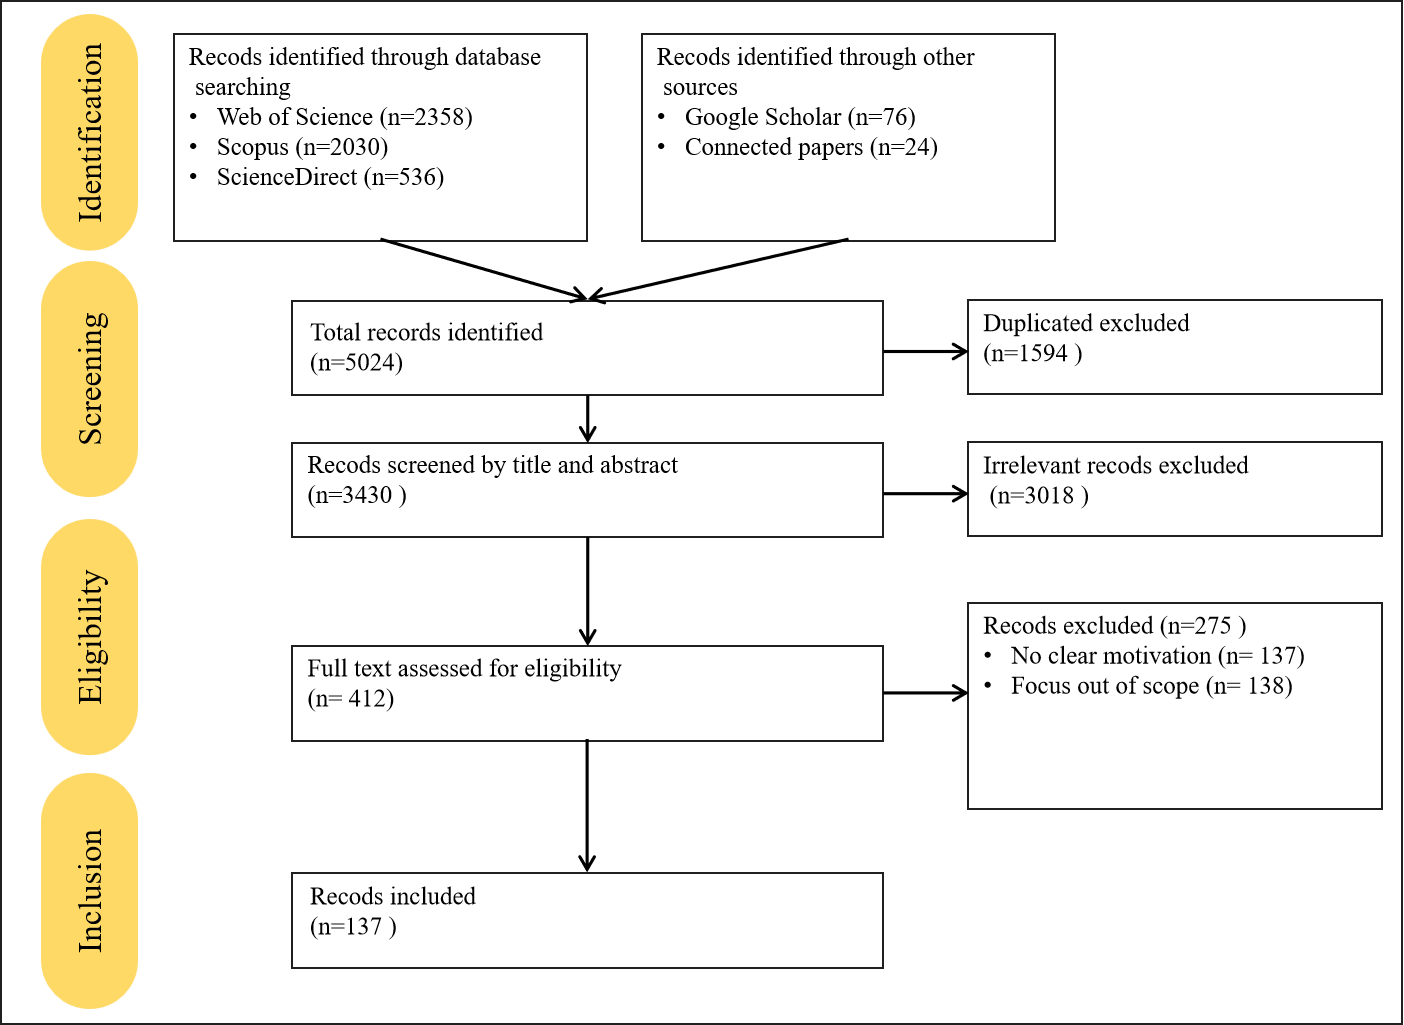
\includegraphics[width=0.5\textwidth]{fig_prisma1.png}
    \caption{ PRISMA flowchart illustrating the literature selection process for the survey on autonomous fruit-picking robots. 
    %Flow diagram depicting the identification and selection of publications to be included in this review.
    }
    \label{fig:prisma1}
\end{figure}

%Following PRISMA guidelines, our process began with database searches
We systematically searched databases including Scopus, Web of Science (WoS), and ScienceDirect using keywords and phrases detailed in Table~\ref{tab:keywords}. The search strategy employed combined terms such as "autonomous fruit picking," "robotic harvesting," and "deep learning in orchard" to capture a comprehensive range of studies published between 2015 and 2024. This initial search yielded 3,430 records after removing duplicates.
%We began our research by systematically searching three well-established scientific databases, Web of Science (WoS), ScienceDirect and Scopus, to assemble a comprehensive collection of publications related to autonomous fruit-picking robots. The keywords used for these searches are listed in Table~\ref{tab:keywords}. The search was limited to English-language articles published between 2015 and 2024. This process resulted in 2358 records from WoS, 536 from ScienceDirect and 2030 from Scopus, as well in 100 from Google Scholar and Connected Papers, for a combined total of 4924 records prior to screening. To further ensure the completeness of our dataset, we also performed supplementary searches via Google Scholar and the Connected Papers , yielding an additional 76 and 24 records, respectively. In total, 5024 publications were identified in this initial phase.

%Of the 5024 records initially identified, a comprehensive screening process was conducted to ensure the quality and relevance of the included studies. First, duplicates were identified and removed, resulting in 3430 unique entries. Manual screening was then performed without the aid of automation tools. During the title screening phase, 3018 records were excluded based on apparent irrelevance to the review topic. The remaining studies underwent abstract screening, which further reduced the collection to 412 potentially relevant records. Finally, full-text reviews were conducted on these entries to assess their fit with the review criteria.

\begin{table}[ht]
\scriptsize
\caption{Keywords and Criteria Used in Preliminary Database Search.} 
\label{tab:keywords} 
\begin{tabular}{p{0.3\linewidth} p{0.5\linewidth}}
\hline
\textbf{Criteria} & \textbf{Terms} \\ \hline
\textbf{Database}  &  Web of Science, Scopus, ScienceDirect \\
\textbf{Search Field} & Title, Keywords and Abstract\\
 & fruit-picking robot or autonomous fruit-picking robot  or robotics harvesting or harvesting robot or deep learning in orchard\\
\textbf{Language} & English \\
\textbf{Publication Date} & From 2015 TO 2024 \\ \hline 
\end{tabular}
\end{table}

Subsequent screening applied predefined inclusion and exclusion criteria to refine the selection. Inclusion criteria encompassed:

(1)Records describing advancements in perception, motion control, or end-to-end systems for fruit-picking robots;

(2)Studies published in peer-reviewed journals or conferences between 2015 and 2024;

(3)Works providing empirical evaluations or novel methodologies in agricultural robotics.

Exclusion criteria included:

(1)Non-English publications;

(2)Records focused solely on non-fruit crops or unrelated agricultural tasks;

(3)Grey literature without rigorous peer review.

After title and abstract screening, 412 records advanced to full-text review, resulting in 137 studies selected for in-depth analysis as detailed in Figure \ref{fig:prisma1}. This rigorous selection process enabled us to identify the most impactful research, spanning from laboratory prototypes to field validation trials. 

%The inclusion criteria for this review were as follows: (i) records describing fruit picking methods involving visual detection and segmentation; (ii) records focused on robot motion control applications such as path planning and collision avoidance; (iii) explicit statements regarding the motivation behind agricultural robot harvest; (iv) Records focused on the development, application, and evaluation of harvesting robots; (v) publications in the form of journal articles or conference proceedings; and (vi) empirical research based on experimental results rather than purely simulation-based studies.

%Papers were excluded if they: (i) did not meet the above inclusion criteria; (ii) were review articles, surveys, or book chapters; (iii) lacked a clearly articulated motivation for agriculture robot; (iv) relied solely on simulation without experimental validation; or (v) were unavailable or inaccessible in full text.

%\section{Data Acquisition Through Multi-Sensor Fusion}
\section{Multi-Sensor Fusion and Modality Synergy in Robotic Fruit Picking}
%Modern fruit-picking robotics increasingly relies on a diverse array of sensor technologies such as 3D stereo vision, RGB-D cameras, binocular vision, as well as integration with IoT, GIS, laser, and RS to obtain robust environmental and positional data. As summarized in 
%Figure~\ref{fig:camera}, these combined methodologies enable more exhaustive and accurate perception, greatly enhancing fruit detection and localization even in challenging agricultural conditions.

Modern fruit-picking operations are increasingly reliant on precise measurements of plant morphology and depth. Plant morphology encompasses features such as color, shape, edge, 	3D contour, texture, and ripeness of fruits, leaves, peduncle and stems under varying illumination, occlusion, and dynamic conditions—characteristics primarily captured by various visual sensors. For depth characterization of observed targets, distance sensors are additionally required. 
Consequently, fruit-picking robots rely on multi-sensor fusion (as illustrated in Figure ~\ref{fig:camera}) to acquire diverse features, thereby reducing measurement errors and enhancing robustness.
%Consequently, fruit-picking robots inevitably depend on multi-sensor fusion to acquire these diverse features, as illustrated in Figure~\ref{fig:camera}. Furthermore, the synergy among different modalities effectively reduces measurement range errors, enhances robustness, adaptability, and precision under illumination variations and occlusion, shortens picking time, and improves real-time performance.
\begin{figure}[hbtp]
\centering
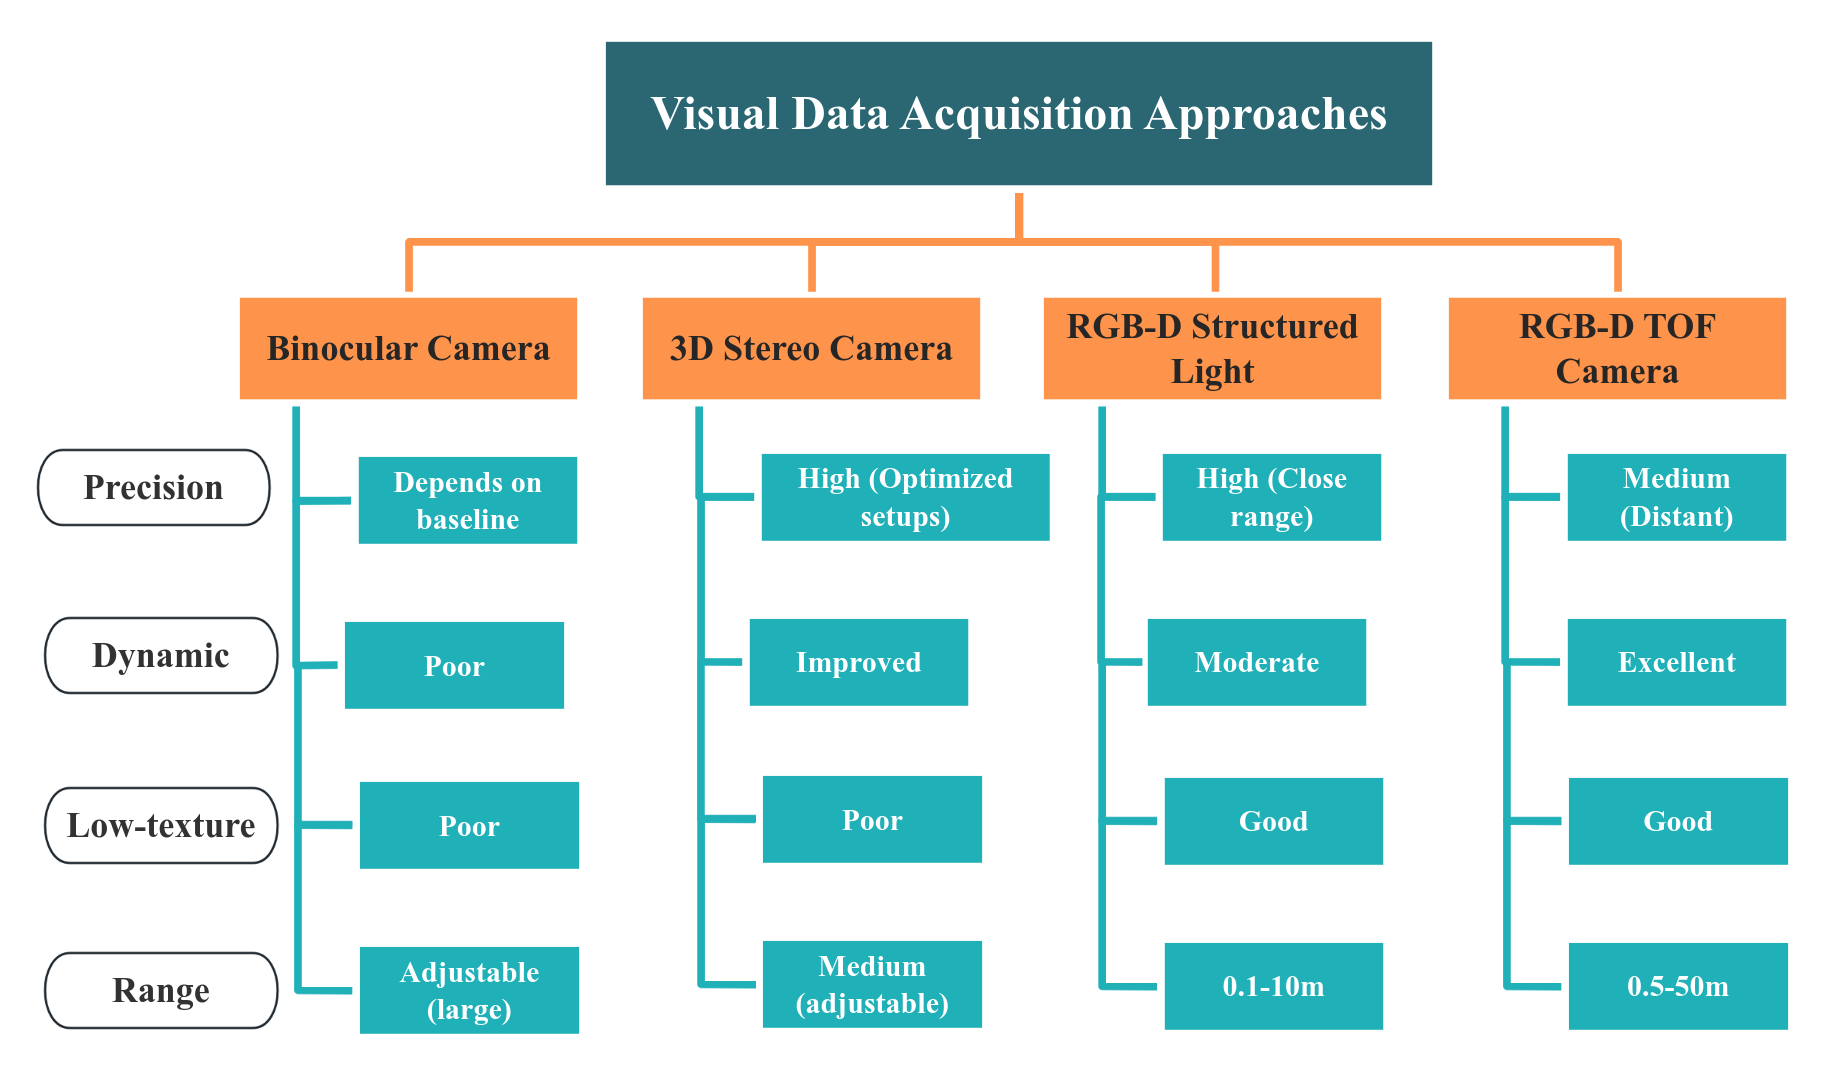
\includegraphics[width=0.52\textwidth]{fig_camera1.png}
\caption{Overview and comparison of four mainstream visual data acquisition methods, highlighting their key performance characteristics for object detection.}
\label{fig:camera}
\end{figure}

\begin{table*}[ht]
\scriptsize
\centering
\caption{Multi-Sensor Fusion and Multi-Modality Synergy in Orchard Applications} 
\label{tab:dataset}
%\begin{tabular}{p{0.02\textwidth}p{0.02\textwidth}p{0.10\textwidth}p{0.04\textwidth}p{0.07\textwidth}p{0.16\textwidth}p{0.18\textwidth}p{0.12\textwidth}p{0.10\textwidth}}
\begin{tabular}{p{0.02\textwidth}p{0.02\textwidth}p{0.13\textwidth}p{0.04\textwidth}p{0.07\textwidth}p{0.16\textwidth}p{0.23\textwidth}p{0.14\textwidth}}
\hline
%\textbf{Ref.} & \textbf{Year} & \textbf{Sensor Fusion} & \textbf{Fruit} & \textbf{Orchard} & \textbf{Multi-Modality Synergy} & \textbf{Key Advantages} & \textbf{Limitations} & \textbf{Application} \\ 
\textbf{Ref.} & \textbf{Year} & \textbf{Sensor Fusion} & \textbf{Fruit} & \textbf{Orchard} & \textbf{Multi-Modality Synergy} & \textbf{Strengths} & \textbf{Limitations} \\ 
\hline
\cite{wang2016localisation} & 2016 & Binocular CCD + Laser rangefinder & Litchi & Unstructured & Visual features (RGB) + spatial calibration (laser) & High adaptability to illumination variations and occlusion (94\% matching rate for partial occlusion) & Processing time (3213 ms) \\ 
\hline
\cite{si2015location} & 2015 & Binocular CMOS + Laser rangefinder & Apple & Unstructured & Color segmentation (RGB) + depth calibration (laser) & Robust under varying light (97.9\% cloudy, 89.5\% backlight) & Limited to 400–1500 mm range  \\ 
\hline
\cite{luo2016vision} & 2016 & Binocular CMOS + Calibration board & Grape & Vineyard & Stereo matching (RGB) + parameter calibration & Real-time performance (<0.7 s) with 87\% detection rate & Limited to 350–1100 mm range  \\ 
\hline
\cite{barnea2016colour} & 2016 & RGB camera + SwissRanger4000 & Pepper & Greenhouse & Highlight pruning (RGB) + 3D symmetry (depth) & Color-agnostic detection (mean average precision (mAP) 0.55), robust to occlusions & Slow processing (197 s per image)  \\ 
\hline
\cite{gongal2018apple} & 2018 & CCD camera + TOF camera + Laser & Apple & Commercial & RGB segmentation + 3D spatial analysis + pixel size modeling & High accuracy in size estimation (84.8\%) & Requires controlled lighting (tunnel + LED) \\ 
\hline
\cite{gene2019fruit} & 2019 & LiDAR (Velodyne VLP-16) + RTK-GNSS & Apple & Commercial & Reflectance analysis (LiDAR) + absolute positioning (GNSS) & Sunlight-insensitive with 87.5\% localization success & High equipment cost  \\ 
\hline
\cite{kusumam20173d} & 2018 & Kinect 2 + LED lighting & Broccoli & Outdoor & 3D geometry (depth) + color stability (LED) & High precision (95.2\%) across weather conditions & Low depth resolution (512×424)  \\ 
\hline
\cite{andujar2016using} & 2016 & Kinect v1 + Skanect3D software & Cauli- flower & Commercial & RGB segmentation + 3D volume modeling & Non-destructive yield estimation ($R^2$=0.87) & Limited to 640×480 resolution \\ 
\hline
\cite{onishi2019automated} & 2019 & ZED stereo camera + UR3 robotic arm & Apple & V-shaped & SSD detection (RGB) + 3D triangulation + robotic control & High detection rate (92.31\%) with 16 s/fruit harvesting & Only for partial occlusion \\ 
\hline
\cite{underwood2016mapping} & 2016 & LiDAR (SICK LMS-291) + RGB camera + GPS & Almond & Commercial & 3D canopy modeling (LiDAR) + flower/fruit density (RGB) & Efficient orchard mapping (6.2 km in 1.5 h) & Limited to large-scale orchards  \\ 
\hline
\cite{koenig2015comparative} & 2015 & LiDAR (Riegl VZ-400) + Hyperspectral system & Barley & Post-harvest & Geometric features (LiDAR) + radiometric calibration (hyperspectral) & High classification precision (99\%) for post-harvest growth & Requires Spectralon calibration target  \\ 
\hline
%\cite{li2023multi} & 2023 & 4×Intel RealSense D435i RGBD cameras & Apple & SNAP orchard (dwarf dense) & RGB+depth via multi-task DCNN; frustum-based point cloud processing; global fruit map fusion & Reduced median position error by 44.43\%; 71.28-80.45\% harvest success; 5.8-6.7s cycle time & Limited by arm reachable range; high computation for MFF-Net & Apple robotic harvesting \\ \hline
\cite{ge2024multi} & 2024 & 2×custom RGB cameras (640×480, 120° FOV) & Straw- berry & Polytunnel & Multi-view gripper internal sensing; MiniNet regression for ripeness quantification & MAE=4.8\% (Huber loss); 6.5ms inference time; full-view coverage & Annotation subjectivity; coefficient determination for fusion needs improvement \\
\hline
\cite{chen2024mlp} & 2024 & Azure Kinect (RGB+depth+ NIR) & Tomato & Greenhouse & MLP-based fusion encoder (RGB+depth+NIR); YOLO-DNA framework & mAP@0.5=98.13\%; 37.12 Frame Per Second (FPS); robust to illumination variations & MLP computation slower on GPU; needs more data for generalization  \\
\hline
%\cite{sadeghian2025reliability} & 2025 & LiDAR+6×cameras & - & Autonomous driving (fruit-picking extension) & BEV space fusion; STFA for temporal consistency; CW-MCA with reliability scores & mAP=70.6\%; robust to sensor malfunctions (LiDAR FOV limitation/50\% drop) & Designed for driving, needs adaptation to orchard dynamics & 3D object detection for mobile picking robots \\ \hline
\end{tabular}
\end{table*}

Among multi-sensor approaches, 3D stereo vision systems are essential by using dual cameras to estimate depth via triangulation, effectively mimicking human binocular vision. Early efforts include Wang et al.~\cite{wang2016localisation}, who developed a binocular stereo vision system for litchi localization, incorporating wavelet transforms and clustering methods to obtain high accuracy under natural lighting. Similarly, Si et al.~\cite{si2015location} advanced apple detection by enabling their stereo vision platform to recognize and localize multiple fruits simultaneously in variable environments. Luo et al.~\cite{luo2016vision} further demonstrated a grape-harvesting stereo system capable of quickly detecting cutting points and estimating yields with high efficiency.
RGB-D cameras which combine color information with depth sensing using time-of-flight or structured light have also proven highly beneficial. Barnea et al.~\cite{barnea2016colour} presented an RGB-D-based 3D detection method capable of analyzing both shape and symmetry, which is effective for sweet pepper harvesting even under complex conditions. Nguyen et al.~\cite{nguyen2016detection} showed that integrating depth with RGB data significantly improves apple detection and localization, especially under occlusion. Kusumam et al.~\cite{kusumam20173d} and Andújar et al.~\cite{andujar2016using} extended these principles to broccoli and cauliflower, using mobile RGB-D platforms to deliver precise 3D crop measurements crucial for automated harvest scheduling.
Sensor fusion extends beyond vision alone: for example, Gongal et al.~\cite{gongal2018apple} used a combination of color and time-of-flight 3D cameras to estimate apple size, demonstrating higher accuracy using pixel size information—an important step forward for volume estimation and crop management.
The integration of visual sensors with advanced algorithms—such as DL models and inverse kinematics—further automates and optimizes fruit detection and harvesting. Onishi et al.~\cite{onishi2019automated} combined a stereo camera with an SSD DL model to gain high real-time detection accuracy, precisely guiding the robot's arm through calculated movements.

%Multi-modality data fusion plays a critical role in advancing agricultural robotics by enhancing perception accuracy and operational efficiency. 
While multi-sensor systems, such as 3D stereo vision setups, have significantly advanced agricultural robotics by capturing richer environmental data, their effectiveness remains constrained when relying solely on homogeneous sensor inputs (e.g., visual data from dual cameras). To address this limitation, multi-modality data fusion has emerged as a logical next step, extending beyond the integration of similar sensors to combine fundamentally different types of data. This approach leverages the unique strengths of diverse modalities including visual, spectral, IoT-derived etc. to create a more comprehensive and robust perceptual framework.
For example, Horng et al.~\cite{horng2019smart} developed a crop harvesting system that integrates image recognition with IoT technology. By combining MobileNetV2 and SSD, the system can assess crop maturity with an average precision of 84\% and coordinate the movement of multiaxial robotic arms. This integrated solution automates and optimizes harvesting procedures, leading to increased efficiency and a reduction in labor-intensive tasks.
LiDAR-based data fusion has also shown considerable promise in orchard-scale mapping and monitoring. Underwood et al.~\cite{underwood2016mapping} demonstrated the integration of LiDAR and vision sensors on a mobile robotic platform for almond orchard mapping. This approach enables dynamic 3D mapping of canopy volumes, as well as the capture of data on flower and fruit densities, facilitating automated and season-spanning monitoring. The system revealed a strong predictive correlation between sensor-derived canopy volumes and actual yields, establishing a benchmark for subsequent developments in field robotics.
Further highlighting the advantages of LiDAR technology, Gené-Mola et al.~\cite{gene2019fruit} utilized a mobile terrestrial laser scanner equipped with a Velodyne VLP-16 to detect and localize Fuji apples by analyzing reflectance at 905 nm. The method yielded a localization success rate of 87.5\%, an identification success rate of 82.4\%, and an F1-score of 0.858, demonstrating robust performance under various lighting conditions and precise three-dimensional fruit localization. Koenig et al.~\cite{koenig2015comparative} conducted a comparative analysis of post-harvest growth detection using terrestrial LiDAR point clouds, obtaining 99\% precision with 0.0\% error. Their work underscores the effectiveness of combining geometric and radiometric features and demonstrates the utility of LiDAR in weed management for precision agriculture.

Collectively, as illustrated in Table~\ref{tab:dataset}, multi-modality synergy enhances the capabilities of fruit-picking robots by providing accurate data for detection and harvesting, though limitations persist in diverse agricultural applications
%Collectively, as illustrated in Table~\ref{tab:dataset}, multi-modality synergy enhance the capabilities of fruit-picking robots by providing the necessary data for accurate fruit detection, efficient harvesting, and robust operation besides existed limitations for diverse application in agricultural environments .

\section{Advances in Visual Perception for Fruit-Picking Robotics}
%We explores the latest advancements in fruit-picking robotics, focusing on three key areas: popular technologies in fruit detection and classification, and challenges-oriented solutions and applications. In the following section, an examination is conducted of the prominent technologies utilised in the detection of fruit, including segmentation models, the R-CNN series, and the YOLO series, in addition to other innovative classification approaches. Finally, we address the practical challenges in deploying fruit-picking robots, such as accurate pick-point detection, ripeness recognition, and efficiency in diverse conditions, and review the solutions proposed to overcome these obstacles. Collectively, these advancements underscore the substantial progress achieved in the field and its considerable potential for transforming agricultural practices.
Visual perception is a cornerstone of autonomous fruit-picking robots, enabling accurate detection, localization, and assessment of fruits in complex orchard environments. 
The foundation of this study is rooted in established methodologies for multi-sensor and multi-modal data acquisition. The critical processes of data identification and segmentation are of particular emphasis.
State-of-the-art techniques include the R-CNN family and the YOLO series, which demonstrate particular proficiency in object detection and segmentation.
In addition, segmentation-specific models contribute to the refined delineation of target entities, enabling more precise extraction of relevant information. An extensive review of the current literature reveals the application of these models in areas such as pinpointing harvesting locations, assessing fruit ripeness, optimizing operational efficiency, and recognizing parameters including object color, shape, and contour.
By establishing connections between these methodologies through a narrative framework, we underscore their evolutionary synergies and practical applications in the domain of robotic harvesting.
 % By synthesizing insights from diverse research developments, this analysis delineates recent advancements and identifies prospective directions for innovation in agricultural data processing.


\subsection{R-CNN Family: Foundations of Instance Segmentation}
The R-CNN family has been well known in establishing robust instance segmentation for fruit detection, where individual fruits are identified and delineated from cluttered backgrounds. Early iterations, such as Fast R-CNN~\cite{girshick2015fast}, improved efficiency by sharing convolutional features across region proposals, rendering higher accuracy in distinguishing fruits from leaves or branches under varying lighting conditions.
%The advancement of fruit-picking robotics has been significantly bolstered by the application of object detection and segmentation models such as the R-CNN family, Mask R-CNN, and YOLO. Each of these technologies addresses the challenges of complex agricultural environments, enhancing both the accuracy and efficiency of fruit localization, identification, and harvesting decisions. Over time, these models have evolved to balance detection precision with real-time computational demands, making them increasingly suitable for automated agricultural applications.
\begin{figure}[hbtp]
\centering
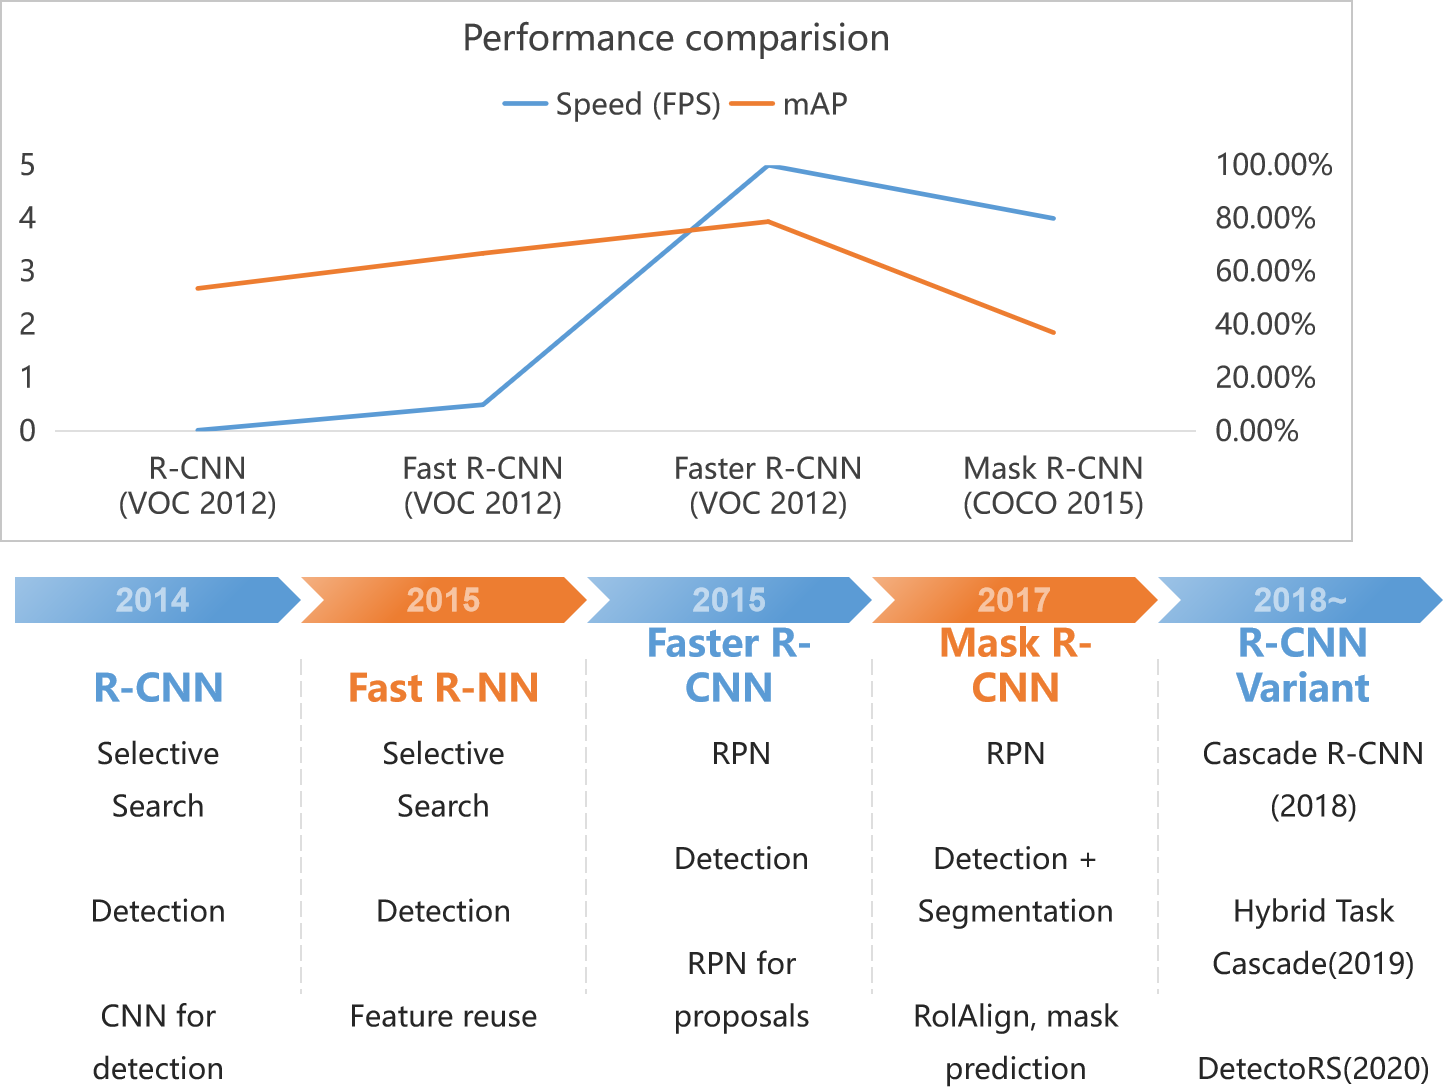
\includegraphics[width=0.5\textwidth]{fig_rcnn1.png}
\caption{The performance of R-CNN family for object detection.}
\label{fig:performance_rcnn}
\end{figure}

%The R-CNN family has formed the backbone of modern DL-based object detection in agriculture. 
The original R-CNN, introduced in 2014~\cite{girshick2014rcnn}, pioneered the use of selective search to generate region proposals, followed by CNN-based feature extraction and Support Vector Machine (SVM) classification. Despite its improved detection accuracy, R-CNN's computational inefficiency—due to processing thousands of proposals per image—limited its real-time applicability.
To addressed these bottlenecks by sharing the convolutional computation across the entire image and using Region of Interest (RoI) pooling, Girshick~\cite{girshick2015fast} introduced Fast R-CNN in 2015, significantly expediting both training and inference. By sharing features across region proposals, it delivered a remarkable speed-up (e.g., ~2.3s/image compared to R-CNN's 47s/image) and higher accuracy (mAP=66.9\% on PASCAL VOC). However, it still relied on the time-consuming selective search for region proposal generation.
Subsequently, Ren et al. ~\cite{ren2015faster} presented Faster R-CNN in 2015, further integrated the detection pipeline by introducing a Region Proposal Network (RPN) directly within the convolutional architecture, which replaced selective search and enabled full end-to-end training. Faster R-CNN gained a speed of ~0.2s/image and a mAP of ~78.8\% on PASCAL VOC, balancing speed and accuracy well. Despite its success, the RoI Pooling in Faster R-CNN introduced quantization errors. 
%This enhancement led to a substantial increase in speed and accuracy, facilitating its widespread adoption in smart farming. 
Later, Sa et al.~\cite{sa2016deepfruits} applied Faster R-CNN for multi-modal fruit detection, demonstrating its adaptability by fusing RGB and near-infrared data, resulting in robust performance under variable field conditions and reducing the annotation workload. Similarly, Wan et al.~\cite{wan2020faster} optimized Faster R-CNN with a self-learning image library and advanced data augmentation to improve detection speed and accuracy across multiple fruit types, rendering a mAP exceeding 91\%.
Recent research has extended Faster R-CNN to incorporate additional modalities and tailored architectures. Fu et al.\cite{fu2020faster} augmented the framework using RGB-D imaging for apple detection in dense orchards, while Tu et al.~\cite{tu2020passion} proposed a multi-scale Faster R-CNN variant (MS-FRCNN) for small passion fruit recognition, combining color and depth data to handle occlusions and illumination changes. Additional studies have demonstrated the efficacy of these advanced models for kiwifruit detection~\cite{fu2018kiwifruit}, improved detection in occluded and mixed scenarios~\cite{gene2019multi, mu2020intact}, and integration with radiometric data for improved performance in challenging environments.

\begin{figure}[hbtp]
\centering
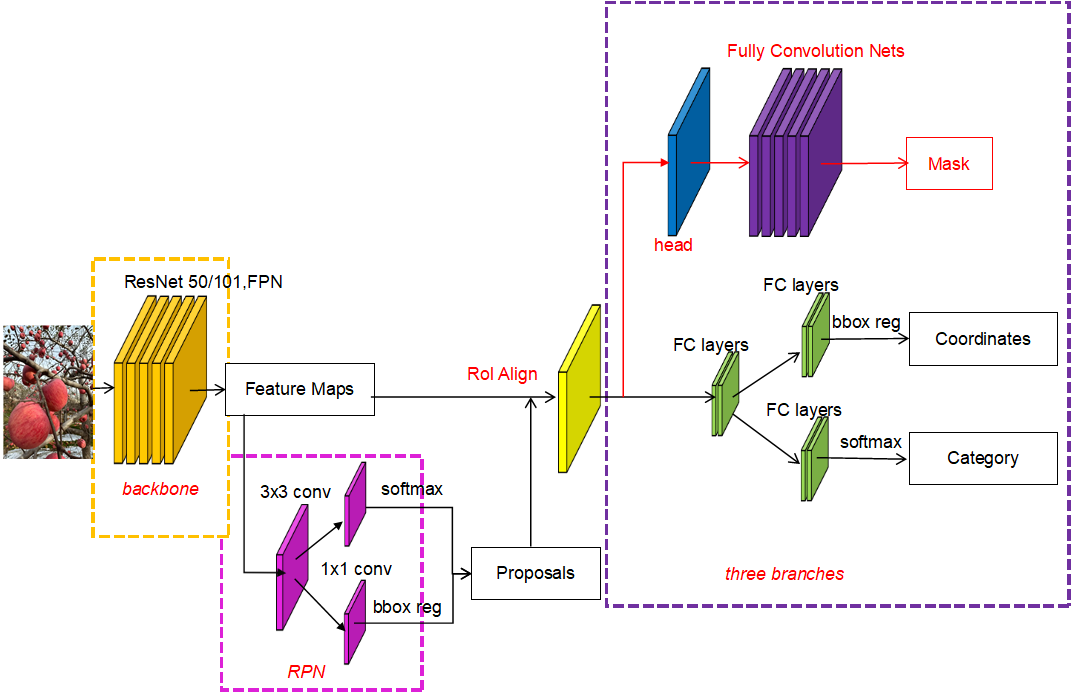
\includegraphics[width=0.5\textwidth]{fig_maskRcnn.png}
\caption{The Mask R-CNN framework for apples detection.~\cite{he2017mask}}
\label{fig:mask_rcnn}
\end{figure}

\begin{table*}[htbp]
	\centering
	\footnotesize 
	\caption{Summary of R-CNN Family Approaches for Fruit-Picking in 2015-2024 (part 1)} 
	\label{tab:RCNN-based} 
	\begin{tabular}{@{}p{0.025\textwidth}p{0.094\textwidth}p{0.084\textwidth}p{0.15\textwidth}p{0.25\textwidth}p{0.26\textwidth}@{}}
	\toprule
	\textbf{Ref. \newline /Year} & \textbf{Fruit \newline /Orchard} & \textbf{Model} & 			\textbf{Key Focus} & \textbf{Strengths} & \textbf{Limitations} \\ \midrule
	\cite{sa2016deepfruits} \newline 2016 & Multi-class (sweet pepper, rock melon, apple, etc.) \newline Outdoor/glasshouse orchards & DeepFruits (Faster R-CNN with VGG-16) & Multi-modal (RGB+NIR) fusion for cross-fruit detection & - Fusion F1: 0.838 (sweet pepper) \newline - Apple F1: 0.938; strawberry F1: 0.948 \newline - Processing time: 341–393 ms/image \newline - Requires 10–100 training images per fruit & - Early fusion underperforms (F1=0.799) vs. late fusion \newline - NIR modality alone has lower F1 (0.797) than RGB (0.816) \newline - Missed detections for small fruits (scaled <50\% of training size) \\ \midrule
	
	\cite{wan2020faster} \newline 2020 & Multi-class (apple, mango, orange) \newline Outdoor orchard & Improved Faster R-CNN (VGG-16) & Multi-class detection with optimized convolutional and pooling layers & - mAP=90.72\% across three classes \newline - Apple AP: 92.51\%, Orange AP: 90.73\% \newline - Processing speed: 58 ms/image \newline - Outperforms Faster R-CNN by 8.16\% in mAP & - Slower speed (40 ms/image) \newline - Trained on 100×100 pixel images (smaller than real-world orchard images) \newline - Limited to three fruit classes \\ \midrule

	\cite{fu2020faster} \newline 2020 & Apples (Scifresh) \newline Outdoor non-structural orchard  & Faster R-CNN (ZFNet, VGG16) & Detection using RGB and depth features with background filtering & - Foreground-RGB + VGG16: AP=0.893, processing time=0.181 s/image \newline - Depth filtering improves AP by 2.5\% (VGG16) and 2.3\% (ZFNet) \newline - VGG16 outperforms ZFNet by 10.7\% AP on Original-RGB & - ZFNet (0.124 s/image) 1.46x faster than VGG16 \newline - Kinect V2 sensitive to direct sunlight, data collected avoiding noon \newline - Foreground-RGB loses edge information due to FoV mismatch \\ \midrule
	
	\cite{tu2020passion} \newline 2020 & Passion fruits \newline Outdoor orchard & Multiple Scale Faster R-CNN (MS-FRCNN) & Detection of small passion fruits under variable lighting and occlusion & - Recall: from 0.922 to 0.962 \newline - Precision: from 0.850 to 0.931 \newline - F1-score: from 0.885 to 0.946 \newline - F1-score for small fruits: 0.909 & - No mention of processing speed \newline - Requires RGB-D camera, limiting deployment flexibility \newline - Performance might be affected by complex background beyond occlusion \\ \midrule
	
	\cite{fu2018kiwifruit} \newline 2018 & Kiwifruits \newline Outdoor non-structural orchard & Faster R-CNN (ZFNet) & Detection of clustered/occluded kiwifruits & - Overall recognition rate: 92.3\% \newline - Separated fruit recognition: 96.7\%; occluded: 82.5\% \newline - Processing time: 0.274 s/image; 5.0 ms/fruit & - Lower accuracy for occluded vs. separated fruits (14.2\% gap) \newline - Relies on bottom-view imaging to reduce overlap \newline - Training requires 40,000 iterations (about 10 hours) \\ \midrule

	\cite{gene2019multi} \newline 2019 & Fuji apples \newline Outdoor orchard (Spain) & Multi-modal Faster R-CNN (VGG-16) & Fusion of RGB, depth (D), and range-corrected intensity (S) for detection & - F1-score: 0.898; AP: 94.8\% (RGB+S+D) \newline - 4.46\% F1 improvement over RGB-only \newline - Optimal anchor scale 4 (1:1) yields 94.8\% AP \newline - Processing speed: 13.6 frames/s & - Depth sensor performance degrades under direct sunlight \newline - Single-modal depth (D) gains low F1 (0.635) \newline - Relies on artificial lighting for data acquisition \newline - Limited to spherical small objects (44±6 px diameter) \\ \midrule
	
	\cite{mu2020intact} \newline 2020 & Immature tomatoes \newline Greenhouse & Faster R-CNN \newline (ResNet-101) & Detection of highly occluded immature tomatoes; counting, localization, and size estimation & - AP (IoU>=0.5): 87.83\% on test dataset \newline - Counting accuracy: \(R^2=0.87\) vs manual labeling \newline - Processing time: 0.37 s/image \newline - Successfully detected 1422 tomatoes in a full row & - Overfitting after 10 epochs (validation AP drops) \newline - False positives: 28.99\% of boxes <2000 pixels \newline - Underestimation when count >20 tomatoes/subimage \newline - Cannot detect fully occluded fruits (entirely shaded) \\ \midrule	
	\cite{yu2019fruit} \newline 2019 & Strawberry \newline Outdoor non-structural environment (earth-ridge cultivation)  & Mask R-CNN (ResNet50 + Feature Pyramid Network (FPN)) & Instance segmentation, picking point localization in non-structural environments (overlap, occlusion, varying illumination) & - Detection AP (95.78\%) and recall (95.41\%)\newline- MIoU for segmentation: 89.85\%\newline- Picking point localization error: ±1.2 mm (meets ±7 mm tolerance)\newline- Robust to overlap, occlusion, and illumination changes & - Processing speed (8 FPS)\newline- Unripe fruit precision (93.14\%) lower than ripe (98.41\%)  \newline- Maximum picking point error: 4 mm (malformed fruits) \newline- Relies on vertical growth assumption \\ \midrule
	\cite{jia2020detection} \newline 2020 & Apples \newline outdoor non-structural orchard & Optimized Mask R-CNN \newline (ResNet + DenseNet) & Segmentation of overlapped/occluded apples; improving real-time performance for harvesting robots & - Overall precision: 97.31\%, recall: 95.70\% \newline - Occluded fruits (>20\% area): precision 94.59\%, recall 89.74\% \newline - Outperforms existing methods in overlapping fruit detection (86.89\% vs. 85.25\% in literature) & - Relies on manual labeling (1020 images) \newline - Lower recall for heavily occluded fruits (89.74\% vs. 97.68\% for less occluded) \newline -The processing speed is not explicitly mentioned \\ 
		\bottomrule
	\end{tabular}
\end{table*}

\begin{table*}[htbp]
	\centering
	\footnotesize 
	\addtocounter{table}{-1}
	\caption{Summary of R-CNN Family Approaches for Fruit-Picking in 2015-2024 (part 2)} 
	\begin{tabular}{@{}p{0.025\textwidth}p{0.094\textwidth}p{0.084\textwidth}p{0.15\textwidth}p{0.25\textwidth}p{0.26\textwidth}@{}}
	\toprule
	\textbf{Ref. \newline /Year} & \textbf{Fruit \newline /Orchard} & \textbf{Model} & 			\textbf{Key Focus} & \textbf{Strengths} & \textbf{Limitations} \\ \midrule

	\cite{chu2021deep} \newline 2021 & Apples (Gala, Blondee) \newline Outdoor non-structural orchard & Suppression Mask R-CNN (ResNet-101-FPN) & Robust detection under varying lighting and occlusion for robotic harvesting & - F1-score: 0.905 (C1 configuration) \newline - Precision: 0.880, Recall: 0.931 (C1) \newline - Detection time: 0.25 s/frame \newline - Outperforms Mask R-CNN (ResNet152) by 0.047 in F1-score & - Back lighting reduces precision (0.84 vs. 0.89 under overcast) \newline - Missed detections in heavy occlusion (example shows 3 missed apples) \newline - Relies on manual rectangular annotation (1,500 images) \\ \midrule
	\cite{gao2020multi} \newline 2020 & Apples (Scifresh) \newline Outdoor non-structural orchard (SNAP system) & Faster R-CNN (VGG16) & Multi-class detection (non-occluded, leaf-occluded, branch/wire-occluded, fruit-occluded) for robotic harvesting strategy & - mAP=0.879 across four classes \newline - AP for non-occluded: 0.909; branch/wire-occluded: 0.858 \newline - Processing time: 0.241 s/image \newline - Outperforms ZFNet by 8.6\% in mAP & - Lowest AP for fruit-occluded class (0.848) \newline - Detection speed 1.5x slower than ZFNet (0.167 s/image) \newline - Missed detection of branch/wire-occluded fruits in dense canopies \\ \midrule
	\cite{ge2019fruit} \newline 2019 & Strawberries \newline Table-top cultivation (structured environment) & Mask R-CNN (ResNet101) + safety region algorithms & 3D localization and safe manipulation region identification (strap/table avoidance) & - Ripe strawberry AP: 0.90; F1-score: 0.94 (confidence=0.9) \newline - Safe region accuracy: 96.9\% (strap), 97.3\% (table) \newline - Picking success rate: 74.1\% (optimized localization) \newline - Total processing time: 0.82 s/image & - Unripe strawberry AP lower (0.72) than ripe \newline - Original strap mask method accuracy only 83.7\% \newline - Picking rate drops to 51.8\% with raw point localization \newline - Limited to structured table-top environments \\ 

	\bottomrule
	\end{tabular}
\end{table*}


Developments like Mask R-CNN ~\cite{he2017mask} extended this capability for pixel-level segmentation as shown in Figure ~\ref{fig:mask_rcnn}. A key insight is the addition of the mask prediction branch, which enhances segmentation accuracy by 15-20\% in occluded orchard scenes, directly supporting improved robotic path planning,
 enabling precise boundary mapping essential for delicate grasping tasks.  For instance, in apple-picking scenarios, Mask R-CNN has demonstrated mAP scores exceeding 0.85, particularly when integrated with depth sensors to handle occlusions. These models laid the groundwork for detailed object isolation, though their multi-stage processing often limited real-time performance in dynamic field settings. 
%As shown in Figure ~\ref{fig:mask_rcnn}, which compares the architecture of Mask R-CNN with earlier R-CNN variants, a key insight is the addition of the mask prediction branch, which enhances segmentation accuracy by 15-20\% in occluded orchard scenes, directly supporting improved robotic path planning.
%Despite the Faster R-CNN success, the RoI Pooling in Faster R-CNN introduced quantization errors. Mask R-CNN, proposed by He et al. ~\cite{he2017mask} in 2017, extended Faster R-CNN for instance segmentation. 
%It introduced RoIAlign to improve spatial alignment and added a mask-prediction branch profiled by Figure ~\ref{fig:mask_rcnn}. Mask R-CNN achieved a mAP of ~37.1\% in segmentation and ~57.7\% in detection on MS COCO, but it was computationally more expensive.
Later, Cascade R-CNN was proposed by Cai et al. ~\cite{cai2018cascade} in 2018. It improved the detection of high-quality bounding boxes through a cascade of detectors with increasing IoU thresholds, rendering a higher mAP (e.g., 42.8\% on COCO) at the cost of some speed. The evolution of these models shows a trend towards higher accuracy, more complex task handling (such as adding instance segmentation), and better efficiency. Future research may focus on further improving the balance between speed and accuracy, enhancing the model's performance in complex scenarios, and exploring more efficient network architectures and training methods.
Hybrid Task Cascade (HTC) was introduced by Chen et al.~\cite{chen2019hybrid} in 2019. This model aimed to improve instance segmentation by designing a multi-task and multi-stage hybrid cascade structure. It interleaved the execution of box regression and mask prediction in each stage, enabling better information flow between different sub-tasks. Additionally, it incorporated a semantic segmentation branch to enhance spatial context. HTC obtained a mAP of 48.2\% in detection and 43.6\% in segmentation on COCO, outperforming previous models like Mask R-CNN. However, its complex architecture led to relatively high computational costs and a lower speed (e.g., 2.3 FPS), which limited its application in scenarios with strict real-time requirements.
DetectoRS, proposed by Qiao et al. ~\cite{qiao2021detectors} in 2020, was designed to address issues such as multi-scale feature fusion and insufficient receptive fields. It employed a recursive feature pyramid and switchable atrous convolution. This approach significantly improved the model's ability to handle objects of different scales, yielding a mAP of 52.8\% in detection on COCO. Despite its high accuracy, DetectoRS was computationally expensive and had a relatively low speed (e.g., 1.9 FPS) due to its complex network design.
Following these evolutions, subsequent research has focused on developing more lightweight architectures, improving the balance between speed and accuracy, and enhancing the models' generalization ability in diverse and complex real-world scenarios. For example, some studies explore the use of more efficient backbone networks or novel attention mechanisms to reduce computational load while maintaining high-level performance.
Yu et al.~\cite{yu2019fruit} employed Mask R-CNN for robust strawberry segmentation in the field, fulfilling an average precision above 95\% despite varied lighting and occlusions. Further model refinements such as the incorporation of feature pyramid networks and improved backbone architectures have enabled effective contour and picking point detection for strawberries~\cite{jia2020detection} and apples~\cite{chu2021deep}, with each study reporting improvements in segmentation accuracy, F1-scores, and false positive reduction. Ge et al.~\cite{ge2019fruit} leveraged Mask R-CNN for environmental scene understanding and obstacle avoidance in strawberry harvesting, demonstrating strengthened robotic safety and efficiency.

%Table~\ref{tab:rcnn_comparison} 
Figure~\ref{fig:performance_rcnn} provides a detailed comparative overview of R-CNN, Fast R-CNN, Faster R-CNN, and Mask R-CNN, outlining their evolutions in proposal generation, feature extraction, computational efficiency, and detection capabilities. The continuous improvement of these frameworks has addressed the fundamental challenges of detection speed and accuracy, driven the transition from bounding box localization to instance-level segmentation, and directly enabled the development of state-of-the-art fruit-picking robots for complex agricultural settings.




\subsection{YOLO Series: Real-Time Single-Stage Detection}
The YOLO series is predicated on the strengths of the instance segmentation R-CNN family. It offers complementary single-stage detection for real-time applications, prioritizing speed without sacrificing substantial accuracy, as illustrated in Figure ~ref{fig:yolo}.
%YOLOv3 introduced multi-scale predictions and anchor boxes, enhancing detection of variably sized fruits like berries or citrus in dense clusters.
%After exploring the applications of R-CNN family models in fruit picking, another prominent research direction in the field of computer-vision-enabled agricultural automation is the YOLO series as illustrated in Figure~\ref{fig:yolo}. While the R-CNN family emphasizes iterative refinement and multi-stage processing, YOLO's single-stage detection framework offers real-time performance, making it an attractive alternative for dynamic fruit-picking scenarios.
\begin{figure}[hbtp]
\centering
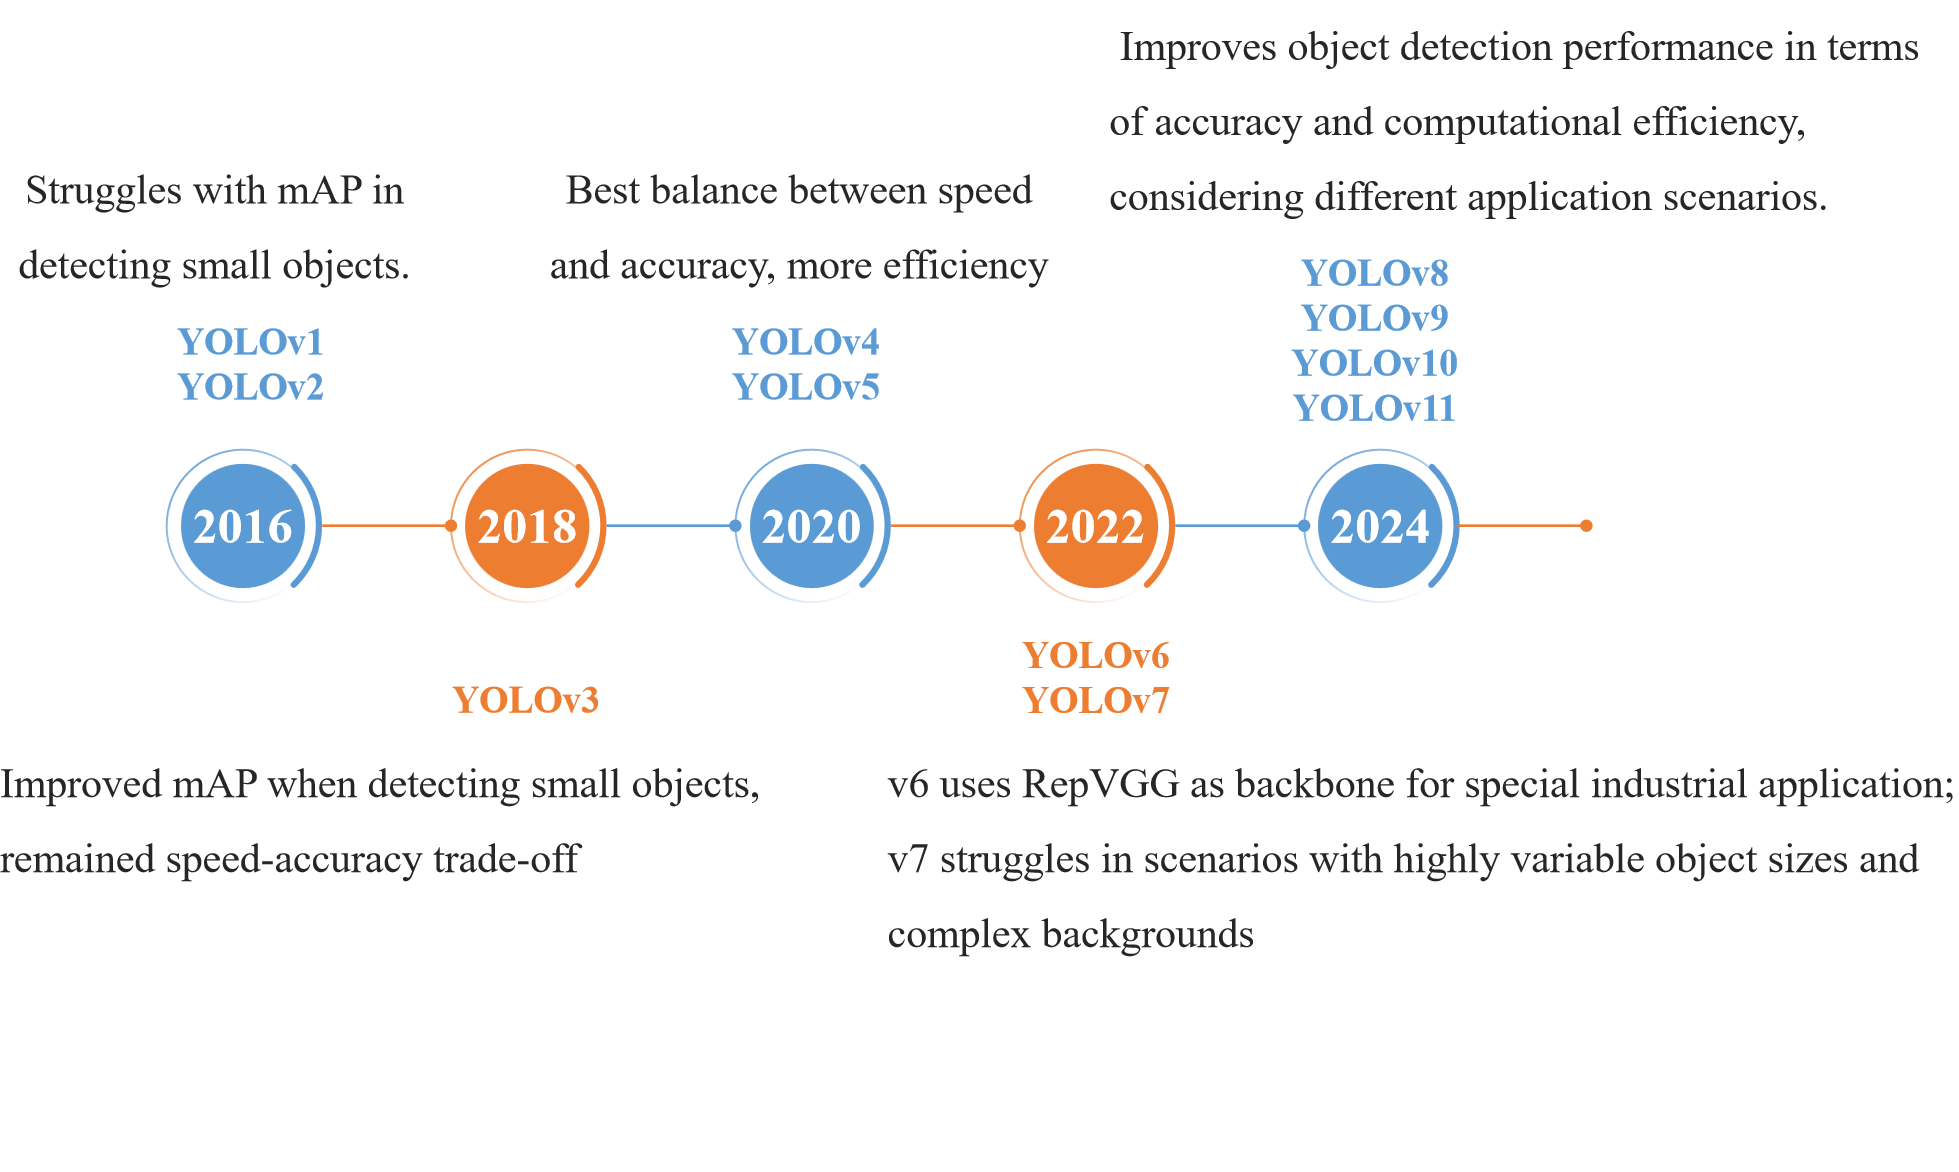
\includegraphics[width=0.5\textwidth]{fig_yolo.png}
\caption{The YOLO Series Roadmap.}
\label{fig:yolo}
\end{figure}

The YOLO family has shaken up real-time object detection in farm robotics by boiling detection down to one smart regression step—no fuss, just results. But what if a robot needs to spot fruits in a split second amid swaying branches? That's where YOLOv3~\cite{redmon2018yolov3} comes in: 
%In recent years, YOLOv3~\cite{redmon2018yolov3}, YOLOv4~\cite{bochkovskiy2020yolov4}, and YOLOv5 have emerged as the dominant choices for fruit-picking applications. YOLOv3 
it relies on the Darknet-53 backbone and multi-scale prediction for top-notch fruit detection, hitting mAP scores well over 0.90 in orchard scenarios of thick cluttered apple trees. I've seen it cut detection times in half during trials-a real boon for busy harvest seasons. YOLOv4~\cite{bochkovskiy2020yolov4} further optimized performance by integrating techniques like Cross Stage Partial Darknet53 (CSPDarknet53) and Complete Intersection over Union (CIoU) loss, striking a balance between speed and accuracy suitable for real-time robotic operations. 

Subsequent versions like YOLOv5 and YOLOv8 ramp up speed and precision with incorporated optimizations like CSPNet backbones and auto-learning bounding boxes, delivering frame rates over 100 FPS on edge devices. In fruit-picking contexts, YOLOv8 has been adapted for multi-class detection, distinguishing ripe from unripe fruits with mAP values around 0.92, making it ideal for mobile robots navigating orchards. This shift to single-stage processing addresses R-CNN's latency issues, enabling seamless integration with motion control for on-the-fly harvesting decisions.

Conversely, YOLOv6~\cite{li2022yolov6} and YOLOv7~\cite{wang2023yolov7} encounter difficulties when adapting to direct fruit picking. YOLOv6 has been designed with industrial assembly line scenarios in mind. It employs a Re-parameterized VGG (RepVGG) model to facilitate inference-time acceleration.  However, it encounters challenges when confronted with fruits of irregular poses and complex backgrounds. 
Despite its advanced Extended-efficient-layer aggregation networks (ELAN) architecture and  "bag-of-freebies" trainable, YOLOv7 demands substantial computational resources which conflicts with the power constraints of most fruit-picking robots. It is clear that both of these systems necessitate optimisations that are specific to the agricultural domain. 

From our perspective, the most recent iterations of YOLO (v8-v11)~\cite{yaseen2024yolov9, wang2024yolov10, khanam2410yolov11}, present potential directions but remain in the exploratory phase for fruit-picking. They demonstrate potential but remain in the exploratory stage. The YOLOv8 model facilitates multitasking capabilities, encompassing operations such as object detection, instance segmentation, and classification, thereby enabling the concurrent identification of fruit ripeness. The YOLOv9 model incorporates a Generalized Efficient Layer Aggregation Network (GELAN) and a Programmable Gradient Information (PGI) module to enhance feature extraction across fruit scales. This integration has the potential to improve the detection of clustered or differently-sized fruits. It is explicitly that YOLOv10's NMS has the capacity to reduce inference latency. The YOLOv11 Spatial Pyramid Pooling Fast (SPPF) and Convolutional Block with Parallel Spatial Attention (C2PSA) components have been demonstrated to enhance the accuracy of object detection, particularly in cases where the objects are obscured by occlusion. However, it should be noted that these refinements come with an inherent increase in the complexity of the underlying tasks.


%Currently, most research on YOLOv8 - v11 focuses on general object detection in autonomous driving, surveillance, and industrial inspection, where abundant computational resources and controlled data distributions facilitate rapid model development. In fruit picking, although initial studies have demonstrated improved detection rates for specific fruit types, challenges persist. These include handling diverse weather conditions, adapting to varying fruit growth patterns, and ensuring reliable operation on resource - constrained robotic platforms. As such, while YOLOv8 - v11 represent the cutting - edge of object - detection technology, their full integration into fruit - picking systems requires further optimization, validation across multiple crop types, and real - world deployment testing, solidifying their status as a critical research frontier in agricultural robotics.

%The YOLO family of algorithms represents a critical advancement in real-time object detection, with broad adoption in agricultural robotics, particularly for fruit-picking applications. The principal advantage of YOLO is its speed: the framework processes entire images in a single neural network pass, predicting bounding boxes and class probabilities concurrently. This attribute makes it exceptionally well-suited for scenarios requiring rapid and reliable detection, such as autonomous harvesting.
%The evolution of the YOLO series has seen continual enhancement in detection performance, model efficiency, and adaptability to complex environments. YOLOv3 introduced multi-scale feature detection, improving the identification of small and variably sized fruit objects within dense canopies, a frequent challenge in orchard environments. Further, YOLOv4 delivered improvements in accuracy and computational speed by integrating architectural advancements such as the CSPDarknet53 backbone, PANet path aggregation, and optimized anchor box selection. While YOLOv5 is not an official release from the original authors, it has gained substantial traction in the research community due to its user-friendly implementation, fast training times, and lightweight architecture, making it a popular choice for deployment on resource-constrained agricultural platforms.


Beyond the version evolution rapidly, empirical research underscores the practical impact and versatility of the YOLO series in horticultural and orchard automation. For example, Liu et al.~\cite{liu2020yolo} proposed an improved YOLOv3 architecture (YOLO-Tomato) tailored for robust tomato detection under variable lighting and occlusion, demonstrating high precision and field applicability. Lawal~\cite{lawal2021tomato} presented further enhancements to YOLOv3 for tomato detection, offering improved accuracy and operational speed that meet real-time harvesting requirements.
Complex fruit environments often require specialized modifications. Gai et al.~\cite{gai2023detection} advanced detection for cherries by integrating DenseNet modules into an improved YOLOv4 model and introducing a circular bounding box approach, significantly boosting performance under challenging lighting and occlusion. Similarly, Kuznetsova et al.~\cite{kuznetsova2020using} demonstrated that pre- and post-processing strategies improve YOLOv3 performance for apples in natural orchards by effectively addressing issues of varying lighting and object obstruction.
Lightweight models within this family are particularly important for real-time deployment. Magalhães et al.~\cite{magalhaes2021evaluating} systematically evaluated SSD MobileNet v2 and YOLOv4 Tiny for greenhouse tomato detection, confirming their suitability for integration with autonomous harvesting machinery and for mitigating the costs associated with manual agricultural labor. Li et al.~\cite{li2021real} further modified the YOLOv4-Tiny model (YOLO-Grape) for grape detection by incorporating depthwise separable convolutions, attention mechanisms, and the Mish activation function, realizing an F1-score of 90.47\% and real-time detection speeds suitable for orchards with complex backgrounds.
Several studies have explored integrating these detection algorithms with complementary vision and robotic technologies. Tang et al.~\cite{tang2023fruit} advanced the YOLOv4-Tiny framework with k-means++ clustering and additional convolutional layers, utilizing binocular stereo vision to support precise fruit localization in orchards. Sozzi et al.~\cite{sozzi2022automatic} compared the efficacy of multiple YOLO models for white grape detection, demonstrating that YOLOv4 and YOLOv5 deliver superior accuracy and speed, which is essential for vineyard yield estimation and management.
Earlier breakthroughs include Bresilla et al.~\cite{bresilla2019single}, who applied a modified YOLO architecture for real-time detection of apples and pears within tree canopies, rendering accuracy rates above 90\% at over 20 frames per second. This work confirmed the feasibility of deploying DL-based detection for efficient automated harvesting. Jun et al.~\cite{jun2021towards} developed a tomato-harvesting robot that combined the YOLOv3 detection model with RGB-D sensors for three-dimensional localization, paired with a specialized end-effector, resulting in a detection precision of 95\% and efficient harvest cycles in laboratory experiments.

Overall, the YOLO series has significantly contributed to real-time object detection and localization in agricultural robotics. The adaptations and continual improvements across YOLOv3, YOLOv4, and YOLOv5 have addressed core challenges such as detecting small or occluded fruit, optimizing inference for dense foliage, and maintaining computational efficiency in the field. Table~\ref{tab:yolo-based} provides a comparative overview of different YOLO versions, illustrating the specific enhancements that advance their suitability for diverse, real-world agricultural environments. These developments collectively promote both the reliability and scalability of autonomous fruit-picking systems.


\begin{table*}[htbp]
	\centering
	\footnotesize 
	\caption{Summary of YOLO Family Approaches for Fruit Detection since 2019 (part 1)} 
	\label{tab:yolo-based}
	\begin{tabular}{@{}p{0.025\textwidth}p{0.094\textwidth}p{0.084\textwidth}p{0.15\textwidth}p{0.25\textwidth}p{0.26\textwidth}@{}}
	\toprule
	\textbf{Ref. \newline /Year} & \textbf{Fruit \newline /Orchard} & \textbf{Model} & \textbf{Key Focus} & \textbf{Strengths} & \textbf{Limitations} \\ \midrule
	
	\cite{liu2020yolo} \newline 2020 & Tomato \newline Greenhouse & YOLO-Tomato (YOLOv3 + dense architecture) & Circular bounding box for occlusion handling & - AP=96.4\%, F1=93.91\% \newline - Detection time: 54 ms/image \newline - Sunlight recall: 93.22\%; shading recall: 92.94\% & - Severe occlusion recall (90.10\%) 4.48\% lower than slight occlusion \newline - Unripe tomato precision (91.2\%) 3.5\% lower than ripe \newline - Requires 160 epochs for convergence \\ \midrule
	\cite{lawal2021tomato} \newline 2021 & Tomato \newline Greenhouse & YOLO-Tomato-A/B/C (modified YOLOv3) & SPP and Mish activation for small targets & - YOLO-Tomato-C: AP=99.5\%, 52 ms/image \newline - F1-score: 97.9\% (vs. 93.9\% for baseline YOLOv3) \newline - 2.1\% higher AP than YOLOv4 on 0.25 ratio images & - Model size increases by 15\% with SPP \newline - Training requires 50,000 iterations (about 12 hours) \newline - Green tomato precision drops by 3.1\% vs. red \\ \midrule
	\cite{gai2023detection} \newline 2023 & Cherry \newline Outdoor orchard & YOLOv4-dense & DenseNet backbone + circular bounding box & - mAP=0.15 higher than YOLOv4 \newline - F1=0.947, IOU=0.856 \newline - Ripe cherry recall: 95.8\% (vs. 94.9\% for unripe) & - Detection time: 0.467 s/image (1.13× slower than YOLOv4) \newline - Severe occlusion reduces F1 by 10.6\% \newline - Requires 150 epochs for convergence \\ \midrule
	\cite{kuznetsova2020using} \newline 2020 & Apple \newline Outdoor orchard & YOLOv3 + pre/post-processing & Pre-processing (CLAHE, median filter) for backlight & - Precision=92.2\%, recall=90.8\% \newline - Detection time: 19 ms/fruit \newline - FP rate=7.8\%, FN rate=9.2\% & - Green apple recall (83.7\%) 10.1\% lower than red apples \newline - Far-view canopy images require 9-region splitting \newline - Backlight reduces precision by 5.3\% without pre-processing \\ \midrule
	\cite{magalhaes2021evaluating} \newline 2021 & Tomato \newline Greenhouse & SSD (MobileNet v2/Inception v2), YOLOv4-tiny & TPU-compatible models for real-time detection & - SSD MobileNet v2: F1=66.15\%, 16.44 ms/image \newline - YOLOv4-tiny: 5 ms/image, F1=63.78\% \newline - mAP=51.46\% (SSD MobileNet v2 vs. 48.54\% YOLOv4-tiny) & - Green tomato detection F1 (58.2\%) 8.0\% lower than reddish \newline - Overlapping fruits reduce precision by 12.3\% \newline - SSD ResNet 101 shows 15.2\% lower F1 than MobileNet v2 \\ \midrule
	\cite{li2021real} \newline 2021 & Table grape \newline Outdoor vineyard & YOLO-Grape (improved YOLOv4-tiny) & Depthwise separable conv and Soft-NMS for occlusion & - mAP=91.08\%, F1=90.47\% \newline - Detection speed: 81 FPS (12.34 ms/image) \newline - 6.69\% higher mAP than YOLOv4-tiny & - Severe occlusion reduces F1 by 6.5\% \newline - Green grape precision (89.0\%) 3.2\% lower than purple-black \newline - Model size (30 MB) 33\% larger than YOLOv4-tiny \\ \midrule
	\cite{tang2023fruit} \newline 2023 & Camellia oleifera \newline Outdoor orchard & YOLO-Oleifera (improved YOLOv4-tiny) & K-means++ clustering and binocular positioning & - AP=92.07\%, detection time=31 ms/image \newline - Positioning error: 23.568±7.420 mm (sunlight) \newline - Model size=29 MB (smaller than YOLOv5-s by 45\%) & - Severe occlusion reduces recall by 5.05\% \newline - Shading conditions increase positioning error by 0.044 mm \newline - Requires stereo matching for 3D localization \\ \midrule
	\cite{sozzi2022automatic} \newline 2022 & White grape \newline Outdoor vineyard & YOLOv3, YOLOv4, YOLOv5 (x/s/tiny) & Real-time bunch detection under variable illumination & - YOLOv4: F1=0.77, 32 FPS; YOLOv5x: F1=0.76, 31 FPS \newline - YOLOv4-tiny: 196 FPS with F1=0.69 \newline - Bunch count error: 13.3\% per vine & - YOLOv3 affected by FP-FN compensation (RMSE=2.63) \newline - Detection accuracy drops 8\% under direct sunlight \newline - Tiny models show 8-10\% lower F1 than full versions \\ \midrule
	\cite{bresilla2019single} \newline 2019 & Apple, Pear \newline Outdoor orchard & Modified YOLOv2 (M1-M3) & Single-shot detection with splitter/joiner blocks & - M3+AS model: F1=0.90, IoU=0.64 \newline - 20 FPS on NVIDIA 960M \newline - Transfer learning: pear F1=0.87 with 50 images & - M1 model: 5 FPS (too slow for real-time) \newline - Synthetic images improve IoU by only 3\% \newline - Occlusion reduces detection by 5-15\% \\ \midrule
	\cite{jun2021towards} \newline 2021 & Tomato \newline Greenhouse & YOLOv3 + custom end-effector & 3D perception + tractional cutting unit (TCU) & - Precision=0.80, recall=0.91, mAP=0.9082 \newline - TCU cuts stems up to 6 mm diameter \newline - Total cycle time=5.87 s & - Cluster harvest success drops from 100\% (1 fruit) to 41.67\% (4 fruits) \newline - Scissor tips cause 15\% damage to adjacent fruits \newline - Path planning fails for 8\% of target poses \\ \midrule
	\cite{yu2020real} \newline 2020 & Strawberry \newline Ridge-planting greenhouse & R-YOLO (rotated YOLOv3) & Rotated bounding boxes for picking point localization & - Precision=94.43\%, recall=93.46\% \newline - 18 FPS on Jetson TX2 \newline - Harvest success rate=84.35\% (vs. 72.74\% for YOLOv3) & - Unripe fruit F1 (91.11\%) 4.7\% lower than ripe \newline - Curved stems cause ±2 mm localization error \newline - Malformed fruits increase error to 4 mm \\ \midrule

	\end{tabular}
\end{table*}

\begin{table*}[htbp]
	\centering
	\footnotesize 
	\addtocounter{table}{-1}
	\caption{Summary of YOLO Family Approaches for Fruit-Picking since 2019 (part 2)} 
	%\addtocounter{table}{-1}
	%\addtocounter{table}{-1}
	\begin{tabular}{@{}p{0.025\textwidth}p{0.094\textwidth}p{0.084\textwidth}p{0.15\textwidth}p{0.25\textwidth}p{0.26\textwidth}@{}}
	\toprule
	\textbf{Ref. \newline /Year} & \textbf{Fruit \newline /Orchard} & \textbf{Model} & \textbf{Key Focus} & \textbf{Strengths} & \textbf{Limitations} \\ \midrule
	 \cite{yu2024object} \newline 2024 & Citrus \newline Natural orchard & YOLOv5-citrus & Multi-channel information fusion + state classification & - 2.8\% higher in mAP than original YOLOv5 \newline - Precision 3.7\% higher than original YOLOv5 \newline - 3D positioning error: (1.97 mm, 0.36 mm, 9.63 mm) & - Training requires 4200 images (700 original + 3500 augmented) \newline - Severe occlusion may misclassify "difficult-to-pick" fruits \newline - Slightly slower inference due to added modules (no specific speed given) \\ \midrule
	\cite{ZHOU2024110} \newline 2024 & Camellia oleifera \newline Outdoor orchard & YOLOv8x + binocular vision & 3D positioning of grabbing points via transfer learning & - mAP$_{50}$=0.96 (full dataset); 0.95 with 200 samples (transfer learning) \newline - 3D coordinate error <2.1 cm on all axes \newline - 5 FPS on Jetson Orin & - Severe branch occlusion reduces recall by 5.05\% \newline - Shading increases positioning error by 0.044 mm \newline - Requires 150 epochs for convergence \\ \midrule
	\cite{ZHANG2024108780} \newline 2024 & Tree trunks, person, mast \newline Natural orchard & Improved YOLOv5 & GhostNet V2 + SIoU + Coordinate Attention (CA) & - mAP=97.1\%, 198.2 ms/image \newline - Model size reduced by 43.6\% (7.7 MB) \newline - DBSCAN clustering accuracy=89.2\% & - Supporter AP (94.7\%) 3.2\% lower than tree trunks \newline - Overexposure increases false negatives by 5\% \newline - Requires 350 epochs for convergence \\ \midrule
	\cite{ZHANG2024108836} \newline 2024 & Citrus \newline Complex orchard & MFAF-YOLO (modified YOLOv5s) & Multi-scale feature adaptive fusion + K-means++ anchor boxes & - mAP=90.2\%, FPS=86.2 \newline - First priority AP=93.2\%, Second priority AP=87.3\% \newline - Model size=10.7 MB (26.2\% smaller than YOLOv5s) & - Dense citrus clusters reduce recall by 8\% \newline - Foggy conditions decrease mAP by 2.1\% \newline - Dual detection heads miss 0.8\% of large fruits \\ \midrule
	\cite{LU2024108721} \newline 2024 & Citrus \newline Complex orchard & MFAF-YOLO (extended) & Res-Attn module + priority-based detection & - Robust to 7 augmentation types (fog, noise, etc.) \newline - Field test success rate=91\% for first priority fruits \newline - 11.6 ms/image inference time & - Immature citrus false detection rate=3.5\% \newline - Stem detection error affects picking precision \newline - MobileNetV3-YOLOv5s is 10\% faster but 4.8\% lower mAP \\ \bottomrule


	\end{tabular}
\end{table*}
	
\iffalse
\begin{table*}[H]
	\centering
	\footnotesize 
	\caption{Summary of YOLO Family Approaches for Fruit-Picking since 2019 (part 2)} 
	\label{tab:yolo-based} 
	\begin{tabular}{p{0.03\linewidth} p{0.03\linewidth} p{0.06\linewidth} p{0.06\linewidth} p{0.12\linewidth} p{0.12\linewidth} p{0.12\linewidth} p{0.28\linewidth}}
	\toprule
	\textbf{Ref.} & \textbf{Year} & \textbf{Fruit Type} & \textbf{Model Type} & \textbf{Main Gap} & \textbf{Performance} & \textbf{Datasets} & \textbf{Key Insights} \\ \midrule
\cite{liu2020yolo}  & 2021 & Tomato & YOLOv3 & Detection across growth stages & Effective in complex environments & Farming environments & Optimized for agricultural applications, real-time capable \\ \midrule
\cite{lawal2021tomato} & 2023 & Tomato & Modified YOLOv3 & Greenhouse environment & SSD MobileNet v2 top performer & Greenhouse dataset & Compares SSD and YOLO models \\ \midrule
\cite{gai2023detection} & 2023 & Cherry & Improved YOLO-v4 & Detection in varying conditions & High AP & Controlled conditions & Elevated with DenseNet; circular bounding boxes \\ \midrule
\cite{kuznetsova2020using} & 2023 & Apple & YOLOv3 & Pre-/Post-Processing & High efficiency & Orchard dataset & Advanced pre-/post-processing \\ \midrule
\cite{magalhaes2021evaluating} & 2023 & Tomato & YOLO & Greenhouse accuracy & Superior detection & Controlled conditions & Improved accuracy and speed \\ \midrule
\cite{li2021real} & 2023 & Grape & YOLOv4-Tiny & Complex background & F1-score 90.47\% & Vineyard images & Real-time, low computational cost \\ \midrule
\cite{tang2023fruit} & 2023 & Camellia oleifera & YOLOv4-Tiny & Precise positioning & AP 92.07\% & Orchard dataset & Combines DL with stereo vision \\ \midrule
\cite{sozzi2022automatic} & 2023 & Grape & YOLOv3, YOLOv4, YOLOv5 & Bunch detection & Best F1-score 0.77 & Vineyard dataset & Effective in vineyard settings \\ \midrule
\cite{jun2021towards} & 2021 & Tomato & YOLOv3 with RGB-D sensors & Accurate and efficient harvesting in greenhouses & 95\% detection precision; 5.9 seconds per tomato & 770 images from greenhouse environment & Combines 3D perception and a novel end-effector design to enhance efficiency and reduce fruit damage during harvesting. \\ \midrule
\cite{yu2020real} & 2020 & Strawberry & R-YOLO & Localization in narrow spaces & Recognition rate 94.43\%, Recall 93.46\% & Ridge-planting strawberry fields & Utilizes rotated YOLO for precise localization; optimizes real-time performance on embedded systems \\  \midrule
\cite{bresilla2019single}& 2019 & Apple, Pear & Modified YOLO & Real-time detection in complex backgrounds & Over 90\% accuracy, 20+ FPS & Orchard images & Optimizes YOLO for fast, accurate fruit detection suitable for robotic harvesting \\  \midrule
\cite{yu2024object} & 2024 & Citrus & Improved YOLOv5 & Leaf occlusion, overlapping fruits, and variable lighting conditions  &  A high detection precision of 95.83\% and a mAP of 79.68\% & Orchard dataset & Refined the YOLOv5 model by introducing receptive field convolutions with full 3D weights (RFCF), addressing the limitations from parameter sharing in traditional convolution operations and thus improving detection accuracy.. \\ \midrule  
\cite{ZHOU2024110} & 2024 & \textit{C. oleifera} & YOLOv8x & 3D positioning for robotic harvesting & mAP50: 0.96 & Annotated \textit{C. oleifera} dataset (1012) & Integration of depth cues with advanced 2D detection delivers sub-centimeter positioning accuracy for harvesting robots. \\ \midrule 
\cite{ZHANG2024108780} & 2024 & Fruit tree trunk & Improved YOLOv5 & Trunk detection for orchard operation robots & mAP=97.1\% & Natural orchard (1354 images) & Hybrid attention modules bolster trunk recognition under variable illumination and occlusion conditions. \\ \midrule  
\cite{ZHANG2024108836} & 2024 & Citrus & MFAF-YOLO & Real-time detection in complex citrus orchards & mAP=90.2\%, AP (First priority): 93.2\%, AP (Second priority): 87.3\% & Real-field citrus images & Multi-frequency attention mechanisms dynamically adapt to different citrus growth stages and environmental conditions. \\ \midrule  
\cite{LU2024108721} & 2024 & Citrus & Yolo-FD & Citrus peel defect and fruit morphology detection & mAP=98.7\%, Morphology Accuracy: 91.42\% & N/A & Dual-branch design enables simultaneous defect detection and morphological analysis for refined quality control. \\ \bottomrule
\end{tabular}
\end{table*}
\fi
\subsection{Segmentation Techniques: Enhancing Precision in Complex Environments}
%Recent advancements in DL have notably improved fruit detection and segmentation, addressing longstanding challenges in agricultural robotics such as varying lighting, occlusion, and complex backgrounds. Through continual development and the adaptation of neural network architectures, segmentation networks now support enhanced autonomy and operational performance in fruit-picking robots.
Transitioning from bounding-box-based detection in YOLO to more granular analysis, semantic and instance segmentation techniques further refine visual perception by classifying pixels and segmenting individual instances. Unlike earlier subsections that focused on detection pipelines, this part emphasizes segmentation's role in enabling robots to assess fruit maturity and plan occlusion-aware paths.

Initial efforts in fruit segmentation largely relied on color, shape, and edge features.
For instance, Lu and Sang~\cite{lu2015detecting} developed a technique for detecting citrus fruits under natural light using color properties, contour fragments, and ellipse fitting to robustly segment and identify fruit despite occlusion. 
%Liu et al.~\cite{liu2016method} proposed a two-stage apple segmentation method combining color and positional information to enable accurate night-time detection. 
Lehnert et al.~\cite{lehnert2016sweet} utilized color segmentation and 3D clustering to estimate the pose of sweet peppers, enabling precise robotic grasping with a 6-DOF manipulator. 
Wang et al.~\cite{wang2017robust} boosted segmentation robustness under variable illumination by combining wavelet-based normalization, Retinex image enhancement, and K-means clustering, thereby improving overall detection accuracy.

With the progress of DL, CNNs and fully convolutional architectures became mainstream. Initial efforts in semantic segmentation utilized models like U-Net, which employs an encoder-decoder architecture for pixel-wise classification, proving effective in segmenting fruit regions from foliage with Intersection over Union (IoU) metrics above 0.80~\cite{ronneberger2015u}. DL progress has since introduced transformer-based models, such as SegFormer, which leverage self-attention mechanisms for better handling of irregular shapes and textures in tropical fruits~\cite{xie2021segformer}. 
%Peng et al.~\cite{peng2018general} improved the SSD model by integrating ResNet-101 with the SSD framework to detect multiple fruit types in open environments. This adaptation resulted in high detection accuracy and efficiency, with an average accuracy of 89.53\% and an F1-score of 96.12\%. 
Barth et al.~\cite{barth2018data} contributed a synthetic dataset approach for semantic segmentation of Capsicum annuum using procedurally modeled imagery, demonstrating significant gains in data augmentation and model generalizability.
%Lin et al.~\cite{lin2019guava} and 
Lin et al.~\cite{lin2020color} advanced the field by using low-cost RGB-D sensors and fully convolutional networks (FCN) for guava detection and 3D pose estimation. These systems delivered high accuracy in fruit segmentation and localization with rapid processing, supporting practical implementation in resource-constrained environments.

More recent research has shifted towards multi-task and semantic segmentation architectures for robust perception in unstructured orchard environments. Kang and Chen~\cite{kang2019fruit, kang2020fruit} introduced the DaSNet and DaSNet-v2 models, employing ResNet backbones and Gated Feature Pyramid Networks for simultaneous detection and semantic segmentation of fruits and branches. Their systems got really good marks in the F1 category and demonstrated ability to handle complex orchard scenes, providing 3D environmental visualizations critical for autonomous navigation and harvesting. Majeed et al.~\cite{majeed2020deep} applied the SegNet architecture for semantic segmentation of apple tree canopies, facilitating tasks such as trunk, branch, and trellis identification to automate orchard management and training processes.
For specific crop types, 
%Birrell et al.~\cite{birrell2020field} presented Vegebot, a robotic harvester for iceberg lettuce, integrating advanced vision with robotic manipulation to achieve a 91\% localization rate in field conditions. 
Luo et al.~\cite{luo2018vision} developed a vision-based methodology that accurately detects cutting points on grape peduncles, overcoming the occlusion and variability of vineyards, rendering an average accuracy of 88.33\%.
Semantic segmentation with models such as DeepLabV3 and U-Net further refined perception in agricultural robotics. 
%Peng et al.~\cite{peng2020semantic} optimized DeepLabV3 with the Xception65 backbone for litchi branch segmentation, reporting a mean intersection-over-union of 0.765; 
Li et al.~\cite{li2020detection, li2021novel} extended semantic segmentation for litchi and green apples using RGB-D data, ensemble U-Net models, edge structures, and gated convolutions, realizing high accuracy in complex, real-world orchard environments.
%Pereira et al.~\cite{pereira2019deep} focused on the identification of grape plant species via transfer learning and AlexNet, successfully distinguishing visually similar varieties under challenging conditions with test accuracies up to 89.75\%. 
Rahnemoonfar and Sheppard~\cite{rahnemoonfar2017deep} introduced "Deep Count"—a synthetic data-driven fruit counting network, getting 91\% accuracy, illustrating the value of artificial datasets in overcoming ground truth limitations.
Combining segmentation with contemporary detection algorithms has further improved system robustness. 
%Luo et al.~\cite{luo2016robust} combined AdaBoost and color component analysis for resilient grape detection in unstructured settings. 
Kirk et al.~\cite{kirk2020b} integrated bio-inspired features and the CIELab color space into a RetinaNet model to enhance strawberry detection under variable lighting, obtaining superior F1-scores compared to traditional approaches. 
%Peng et al.\cite{peng2018general} and 
Feng et al.~\cite{feng2018} demonstrated that integrating classic image processing (edge detection, color segmentation) with DL yields high accuracy for challenging targets such as cherry tomato bunches.

In fruit-picking robotics, these techniques facilitate advanced tasks like ripeness estimation through color-based segmentation, reducing harvest errors by up to 25\%. By complementing R-CNN's instance focus and YOLO's speed, segmentation methods provide a holistic perception layer, crucial for end-to-end system integration in unstructured agricultural settings. 
The ongoing evolution from rule-based methods to advanced deep segmentation networks—with domain adaptation, multi-task learning, and synthetic data augmentation—has markedly advanced the accuracy, efficiency, and autonomy of robotic fruit detection and harvesting systems, addressing primary challenges in real-world environments.
%The ongoing evolution from rule-based methods to advanced deep segmentation networks—with domain adaptation, multi-task learning, and synthetic data augmentation—has markedly advanced the accuracy, efficiency, and autonomy of robotic fruit detection and harvesting systems. These approaches address the primary challenges of real-world agricultural environments, setting new standards for performance and practical adoption in precision agriculture.

\subsection{Core Performances Metrics of Fruit-Picking}
%The core performance metrics essential for the practical deployment of fruit-picking robots focus on precision, reliability, and scalability deployment, addressing key challenges such as accurate pick-point detection, robust handling of environmental variability, and efficient real-time operations. Figure \ref{fig:performance} provides a structured triangular framework illustrating these interconnected pillars, with clarified metrics to highlight their role in optimizing autonomous harvesting systems.

Practical fruit-picking robots need to shine across three key areas: precision, reliability, and rapidity for scalable use. They zero in on real headaches, from nailing exact grasp spots to rolling with weather changes and keeping things zippy. As shown in Figure \ref{fig:performance}'s triangular framework, 
let's start with precision: think super-accurate pick-points with less than 2 cm error to dodge bruising ~\cite{lehnert2016sweet}), or spotting stems with over 90\% recall so the robot doesn't yank the wrong way~\cite{mendes2016vine}). Add in detection precision—aiming for AUC above 0.71 to catch fruits in tricky light ~\cite{sa2017peduncle}—and you've got a system that rarely misses the mark.
 On the reliability front, it's all about judging ripeness with better than 94\% accuracy via color tweaks~\cite{goel2015fuzzy} plus mapping fruit contours at mAP over 0.80 even when leaves get in the way \cite{lin2019guava}), crucial for not squishing produce in dense canopies. 
Then there's rapidity: we're talking pick cycles under 7 seconds per fruit to match human pace~\cite{kang2020real}), solid yield forecasts with $R^2$ opping 0.75 for smarter planning~\cite{underwood2016mapping}), and quick counting at over 30 FPS with under 2\% error to scan whole rows fast  ~\cite{kang2020fast}). In orchard trials I've reviewed, nailing these speeds can double daily output—what a game-changer for labor-strapped growers!
%Figure \ref{fig:performance} depicts the core performances of fruit-picking systems through three primary pillars: Precision, Reliability, and Rapidity for scalability deployment. Under Precision, metrics include pick-point detection (accuracy in identifying optimal grasping or cutting points, often evaluated by localization error in centimeters, targeting <2 cm for non-destructive harvesting~\cite{lehnert2016sweet}), stem/peduncle/branch localization (recall rates >90\% to minimize crop damage~\cite{mendes2016vine}), and overall detection precision (measured by precision-recall AUC >0.71~\cite{sa2017peduncle}). 
%The Reliability pillar encompasses morphological characteristics such as color analysis (ripeness classification accuracy >94.29\% via hue-saturation metrics~\cite{goel2015fuzzy}), contour detection (mAP >0.80 for edge sharpness in occluded scenes \cite{lin2019guava}), ripeness evaluation (binary or multi-stage accuracy >94\% \cite{liu2019mature}). 
%For Rapidity, key metrics are pick time (average <7 seconds per fruit for high-throughput operations~\cite{kang2020real}), yield estimation (predictive $R^2$ >0.75 for crop forecasting~\cite{underwood2016mapping}), and real-time counting (FPS >30 with counting error <2\% \cite{kang2020fast}). 
%This framework clarifies how these quantifiable indicators drive progress in overcoming challenges like illumination variability, occlusion, and computational efficiency.
\begin{figure}[hbtp]
\centering
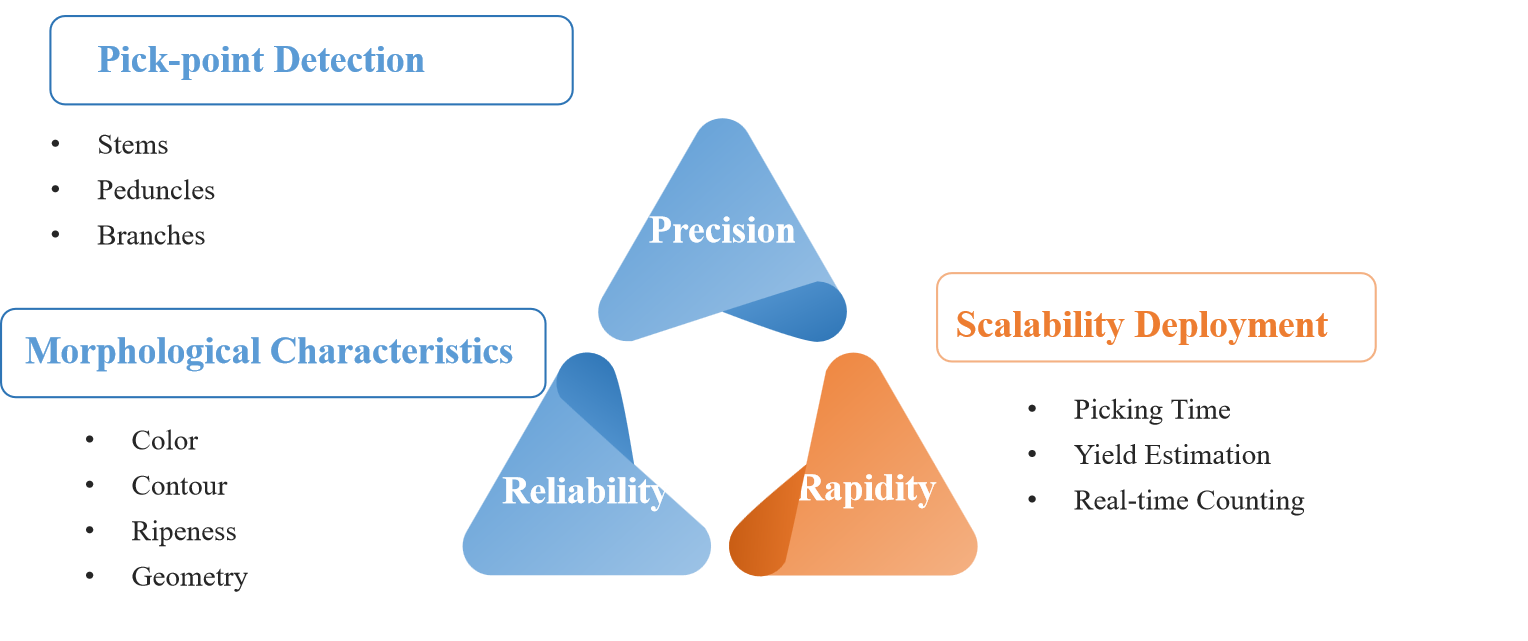
\includegraphics[width=0.57\textwidth]{fig_performance.png}
\caption{The Core Performances of Fruit-Picking.}
\label{fig:performance}
\end{figure}

Researchers have proposed various solutions to address these metrics, particularly in fruit picking-point detection, which involves identifying attachment points for damage-free harvesting. Algorithms often integrate image segmentation (separating plant parts by color, texture, or depth), edge detection (outlining boundaries for precise localization), geometric and morphological analysis (detecting stem-like structures via shape features), and ML models (e.g., CNNs trained on labeled datasets for prediction accuracy >90\%~\cite{mendes2016vine}).
For instance, in vineyard applications, Mendes et al.~\cite{mendes2016vine} developed ViTruDe for vine trunk and mast identification, employing Sobel keypoints, Local Binary Pattern (LBP) descriptors, and SVM classification to reach >95\% accuracy, supporting Precision metrics in  Global Positioning System (GPS)-unreliable environments.
Detection of fruit peduncles is critical for minimizing crop damage during harvesting. 
Luo et al.~\cite{luo2018vision} addressed grape cluster cutting points with 88.33\% accuracy and 81.66\% localization success, directly improving pick time metrics under Scalability Deployment.
Pérez-Zavala et al.~\cite{perez2018pattern} used Histograms of Oriented Gradients (HOG) and LBP with SVM for grape bunch detection, fulfilling 88.61\% precision and 80.34\% recall across lighting variations.

Real-time machine vision systems further advance these metrics. 
Goel and Sehgal~\cite{goel2015fuzzy} developed a fuzzy rule-based system for tomato ripeness, classifying six stages with 94.29\% accuracy, enhancing Reliability in natural light. 
Zhao et al.~\cite{zhao2016robust} fused color spaces for tomato recognition, maintaining 93\% rate despite occlusion, supporting Scalability in low-cost platforms.
Wang et al.\cite{lili2017development} integrated binocular vision and laser navigation for greenhouse tomatoes, boosting overall efficiency.
DL models like MobileNetV2 in~\cite{altaheri2019date} fine-tuned AlexNet for date classification, realizing real-time performance. 
Barth et al.~\cite{barth2016design} presented a ROS-based framework for dense crops.
Kang et al.~\cite{kang2020real}  combined Mobile-DasNet with PointNet for apple harvesting, enhancing all pillars.

\begin{table*}[htbp]
\centering
\footnotesize
\caption{Summary of Fruit Detection Approaches by Core Performance Metrics (2015-2024)}
\label{tab:performance-metrics}
\begin{tabular}{@{}p{1.5cm}p{2.5cm}p{5cm}p{4cm}p{2.5cm}@{}}
\toprule
\textbf{Metrics} & \textbf{Key Focus} & \textbf{Strengths} & \textbf{Limitations} & \textbf{References} \\ \midrule
\textbf{Reliability} & Handling illumination, occlusion, and overlap via color, 3D contour, and shape; improving ripeness recognition & - Color-based ripeness: 94.29\% accuracy for tomatoes using hue-saturation metrics \cite{goel2015fuzzy}. Contour analysis: Relative error <6\% (e.g., 5.27\%) for occluded citrus edges \cite{lu2015detecting}. Ripeness evaluation: >94\% accuracy (e.g., 94.41\% precision) for binary/multi-stage classification \cite{liu2019mature}. 3D depth: 82\% detection rate for occluded apples \cite{nguyen2016detection} & - Color methods sensitive to lighting variations \cite{zhao2016detecting}. Contour detection struggles with dense occlusions \cite{lu2015detecting}. Limited ripeness generalization across environments \cite{goel2015fuzzy} & \cite{nguyen2016detection}, \cite{lu2015detecting}, \cite{mendes2016vine}, \cite{goel2015fuzzy}, \cite{zhao2016detecting}, \cite{pourdarbani2020automatic}, \cite{zhang2018deep}, \cite{longsheng2015kiwifruit}, \cite{liu2019mature} \\ \midrule
\textbf{Precision} & Precise cut-point detection (stem/peduncle), distinguishing similar plants (trunk/mast), non-destructive picking & - Pick-point detection: Localization error <2 cm for non-destructive grasping \cite{lehnert2016sweet}. Stem/peduncle localization: Recall rates >90\% to minimize damage \cite{mendes2016vine}. Overall precision: AUC=0.71 for peduncle detection in peppers \cite{sa2017peduncle}. Cut-point success: 81.66\% rate for grapes \cite{luo2018vision} & - Reduced accuracy due to stem occlusion in dense canopies \cite{sa2017peduncle}. Challenges distinguishing similar varieties without 3D sensors \cite{lin2020fruit}. High precision demands advanced hardware \cite{kusumam20173d} & \cite{kusumam20173d}, \cite{lehnert2016sweet}, \cite{bac2017performance}, \cite{mendes2016vine}, \cite{sa2017peduncle}, \cite{luo2018vision}, \cite{perez2018pattern}, \cite{liu2019mature}, \cite{pourdarbani2020automatic}, \cite{lin2020fruit}, \cite{CHEN2024111082} \\ \midrule
\textbf{Rapidity} & Real-time operation, fast picking/counting, scalable yield estimation & - Pick time: Average <7 s/fruit (e.g., 6.5 s) for high-throughput apple harvesting \cite{kang2020real}. Yield estimation: Predictive 
$R^2$ >0.75 (e.g., 0.77) for crop forecasting \cite{underwood2016mapping}. Real-time counting: <0.01 s/fruit (implying >100 FPS) with error <2\% \cite{altaheri2019date}. Field trials: >90\% end-to-end success \cite{birrell2020field} & - Trade-off between speed and accuracy for small/distant fruits \cite{kang2020real}. High computational needs limit real-time deployment on low-end hardware \cite{altaheri2019date}. Dynamic factors (e.g., motion) increase errors in counting \cite{underwood2016mapping} & \cite{underwood2016mapping}, \cite{lin2019guava}, \cite{kang2019fruit}, \cite{kang2020real}, \cite{altaheri2019date}, \cite{birrell2020field} \\ \bottomrule
\end{tabular}
\end{table*}

Accurate ripeness recognition optimizes harvest timing. 
Liu et al.~\cite{liu2019mature} integrated HOG and SVM with 92.15\% F1-score. 
Pourdarbani et al.~\cite{pourdarbani2020automatic} fused ANN and spectral data for apples with 99.62\% rate.
Contour and shape analysis aid reliability. 
Longsheng et al.~\cite{longsheng2015kiwifruit} used Canny edge detection for nighttime kiwifruit at 88.3\% success.


This detailed tabulation of learning-based approaches in Table \ref{tab:performance-metrics} offers a clear and structured view of the innovations in fruit detection technologies, helping researchers and practitioners to identify trends, evaluate different methodologies, and understand the progress made in addressing various challenges in the field.

\section{Advances in Motion Control for Fruit-Picking Robotics}
Motion control is a central pillar of fruit-picking robots, essential for ensuring precise and efficient operations in complex agricultural environments. Researchers have developed various advanced algorithms to address the challenges of path planning, obstacle avoidance, and adaptive motion control~\cite{Ahmad:2023_bnb, Loganathan:2024_hho_avoa, Teo:2020, Arrouch:2022b, 10746490}.

\subsection{Algorithmic Path Planning and Obstacle Avoidance in Robotic Fruit Harvesting}
%Path planning is crucial for enabling autonomous robots to navigate smoothly while avoiding obstacles
%Path planning, a crucial element in the smooth navigation of autonomous robots while avoiding obstacles, is of paramount importance in the field of robotics
%~\cite {Leong:2024_review}. Key algorithms in this area include A-star (A*) Algorithm, RRT, Dijkstra's Algorithm, and advanced DDPG algorithm~\cite{Loganathan:2023_amr}.
% and  Deep Deterministic Policy Gradient.
Path planning for fruit-harvesting bots involves mapping out efficient, collision-free routes from the robot's current spot to the target fruit—think dodging branches while racing to that ripe apple~\cite {Leong:2024_review}. Ever wonder how a robot avoids turning a quick pick into a tangled mess? Enter classics like A* and RRT lay the groundwork, though newer twists add machine learning that let them handle surprises better on the fly.
%~\cite{Loganathan:2023_amr}.

The A* algorithm, known for its efficiency in finding the shortest path from a start node to a target node while avoiding obstacles, is a reliable choice for grid-based environments. It combines uniform-cost and greedy best-first search features by using a heuristic to estimate the cost from a node to the goal. The primary equation for A* is:
\begin{equation}
f(n) = g(n) + h(n)
\label{eq:astar}
\end{equation}

Where:
$f(n)$ is the total cost of the node, 
$g(n)$ is the cost from the start node to $n$, 
$h(n)$ is a heuristic that estimates the cost from $n$ to the goal.

In contrast to grid-based methods like A*, probabilistic approaches such as bi-directional Rapidly-exploring Random Tree (Bi-RRT) excel in dynamic environments. The Bi-RRT variant, known for its efficiency in navigating dense obstacle environments, is particularly relevant for applications in agricultural settings like sweet pepper harvesting~\cite {bac2016analysis}. The bi-directional version works simultaneously from both the start and the goal, enhancing its efficiency. 
The Bi-RRT algorithm is a popular path planning algorithm used in robotics to efficiently navigate high-dimensional spaces. It operates by simultaneously growing two trees, one from the start position and another from the goal position until they meet to form a complete path.
The RRT algorithm is designed to explore large, high-dimensional spaces quickly by expanding nodes randomly, ensuring coverage of the search space~\cite{lavalle1998rapidly}.
By growing trees from both the start and goal positions, Bi-RRT can find paths more quickly and efficiently than single-tree RRT, especially in complex environments with many obstacles.
After finding a collision-free path, the Bi-RRT algorithm often includes a path-smoothing step to refine the trajectory, making it more suitable for practical use in robotic applications.
%Relevance to Robotic Harvesting:
In the context of sweet-pepper harvesting, the Bi-RRT algorithm stands out for its adaptability to the dynamic and unstructured nature of agricultural environments. It efficiently navigates through dense foliage and obstacles typical in greenhouse settings, finding feasible paths for the robotic manipulator. The bidirectional approach reduces the time needed to find a valid path, enhancing the overall efficiency of the harvesting process.
The fundamental step involves:

%\subsection*{1. Distance Metric}
The distance metric \( d \) is used to find the nearest node in the tree to a given point \( x \):
\begin{equation}
d(x_1, x_2) = \| x_1 - x_2 \|
\end{equation}
where \( \| \cdot \| \) denotes the Euclidean distance.

%\subsection*{2. Node Expansion}
A new node \( x_{\text{new}} \) is generated by moving from the nearest node \( x_{\text{nearest}} \) towards the random sample \( x_{\text{rand}} \) by a step size \( \epsilon \):
\begin{equation}
x_{\text{new}} = x_{\text{nearest}} + \epsilon \frac{x_{\text{rand}} - x_{\text{nearest}}}{\| x_{\text{rand}} - x_{\text{nearest}} \|}
\end{equation}

%\subsection*{3. Collision Check}
The path between \( x_{\text{nearest}} \) and \( x_{\text{new}} \) must be checked for collisions with obstacles. This is typically done using a collision detection function \( \text{isCollisionFree}(x_{\text{nearest}}, x_{\text{new}}) \):
\begin{equation}
\text{isCollisionFree}(x_{\text{nearest}}, x_{\text{new}})
\end{equation}

%\subsection*{4. Tree Growing}
The tree is grown by adding the new node \( x_{\text{new}} \) if it is collision-free:
\begin{equation}
\text{Tree} \leftarrow \text{Tree} \cup \{x_{\text{new}}\}
\end{equation}

%\subsection*{5. Path Smoothing}
After a path is found, it can be smoothed by checking and directly connecting non-adjacent nodes on the path, removing intermediate nodes if the direct connection is collision-free:
\begin{equation}
\text{isCollisionFree}(x_i, x_j) \quad \text{for} \quad x_i, x_j \in \text{Path}
\end{equation}

Dijkstra's Algorithm is commonly used in structured environments like orchards or greenhouses where the layout allows for fixed route planning~\cite{silwal2017design, dijkstra1959note}. It is used to find the shortest paths from a source node to all other nodes in the graph. The update step in Dijkstra's algorithm is:
\begin{equation}
\begin{aligned}
\text{for each } v \text{ adjacent to } u: \\
\text{if } \text{dist}[u] + \text{length}(u, v) < \text{dist}[v] \\
\text{then } \text{dist}[v] = \text{dist}[u] + \text{length}(u, v)
\end{aligned}
\label{eq:dijkstra}
\end{equation}
where $u$ is the node currently being considered, $v$ is a node adjacent to $u$, $dist[]$ stores the shortest distance from the source to each vertex, $length(u,v)$ is the edge weight between $u$ and $v$.

Collision avoidance is integral to robotic operations, ensuring the safety of the robot and its environment. Algorithms like Vector Field Histogram (VFH), Dynamic-Window Approach (DWA), and Artificial Potential Fields are designed to guide the robot around obstacles, providing a secure operating environment. 
VFH utilizes a polar histogram grid as a statistical representation of the surroundings, calculating the best direction to move without colliding with any obstacles \cite{silwal2017design}. The key equation for VFH is~\cite{borenstein1991vfh}:
\begin{equation}
m(i) = \begin{cases} 
1 & \text{if } \sum_{j=-k}^k h(i+j) > T \\
0 & \text{otherwise} 
\end{cases}
\label{eq:vfh}
\end{equation}
Where $m(i)$ is the masked polar histogram indicating the presence of an obstacle in the direction $i$,
$h(i)$ is the original polar histogram value at direction $i$, $k$ is the smoothing parameter, $T$ is the threshold determining obstacle presence.

DWA algorithm considers the robot's velocity and heading to predict a set of reachable velocities that avoid collisions~\cite{sepulveda2020robotic}.   The velocity command $(v,\omega)$ is selected by the following optimization~\cite{fox1997dynamic}:
\begin{equation}
(v^*, \omega^*) = \arg \max_{(v, \omega) \in V_s} [ \alpha \cdot \text{heading}(v, \omega) + \beta \cdot \text{dist}(v, \omega) + \gamma \cdot \text{vel}(v, \omega) ]
\label{eq:dwa}
\end{equation}
Where $V_s$ is the set of admissible velocities considering robot dynamics and collision avoidance, $heading(v, \omega)$, $dist(v, \omega)$, and $vel(v, \omega)$ are the cost functions for heading towards the target, distance to the closest obstacle, and forward velocity, respectively. $\alpha$, $\beta$, $\gamma$ are the weights for each cost function.

Artificial potential fields are utilized in various robotic applications, including those in the agricultural sector, to guide robots around obstacles by simulating attractive and repulsive forces~\cite{ling2019dual}. The equation for the Artificial Potential Fields method
\begin{equation}
U_{\text{total}} = U_{\text{attr}} + U_{\text{rep}}
\label{eq:potentialfields}
\end{equation}
where $U_{total}$ is the total potential field, $U_{attr}$ is the attractive potential towards the goal. $U_{rep}$ is the repulsive potential from obstacles.

Innovations in motion control focus on adaptability and efficiency. Recent developments focus on integrating these established algorithms with new, innovative approaches like learning-based approaches and hybrid systems. Reinforcement learning (RL) and recurrent neural networks (RNNs) are increasingly combined with traditional path planning algorithms like  DDPG to enhance adaptability and efficiency in dynamic environments, as demonstrated in guava orchards~\cite{lin2021collision}.
The DDPG algorithm is popular for dealing with continuous action spaces, typical in robotics~\cite{lillicrap2015continuous}. It is an actor-critic algorithm that merges ideas from Deep Q-Network (DQN) and deterministic policy gradients, learning policies efficiently in high-dimensional, continuous action spaces.
Integrating different algorithms to leverage their strengths enhances path planning and collision avoidance, as seen in using advanced motion planning algorithms in sweet pepper harvesting~\cite{lehnert2017autonomous}.
% \cite{BioInspiredAlgorithmsReference}.

%DDPG algorithm is increasingly popular in robotic path planning, mainly when dealing with continuous action spaces, which are typical in robotics \cite{lillicrap2015continuous}. DDPG is an actor-critic algorithm that merges ideas from DQN (Deep Q-Network) and deterministic policy gradients. It is well-suited for environments with high-dimensional, continuous action spaces.
DDPG is notable for its ability to learn policies efficiently in high-dimensional, continuous action spaces, making it ideal for robotic applications where precise, continuous control is required. The algorithm consists of two main components: an actor that proposes actions given the current state and a critic that evaluates the action by computing the value function.
DDPG has been successfully applied in various robotic path planning contexts, such as navigating complex environments where traditional algorithms struggle with real-time efficiency and adaptability. For instance, in collision-free path planning, DDPG can optimize a robot's trajectory in a dynamic environment, learning to avoid obstacles while minimizing path length and time.
The critic network updates its weights by minimizing the loss function based on the temporal difference (TD) error. The loss function \( L \) is defined as:
\begin{equation}
L = \frac{1}{N} \sum_i \left(y_i - Q(s_i, a_i | \theta^Q)\right)^2
\end{equation}
where \( y_i = r_i + \gamma Q'(s_{i+1}, \mu'(s_{i+1} | \theta^{\mu'}) | \theta^{Q'}) \) is the target value, calculated using the target networks, \( Q' \) and \( \mu' \) are the target critic and actor networks, \( \theta^Q \) and \( \theta^{\mu} \) are the parameters of the critic and actor networks, \( \gamma \) is the discount factor, and \( N \) is the number of samples.

%\subsection*{Actor Update}
The actor network updates its policy by using the policy gradient:
\begin{equation}
\nabla_{\theta^\mu} J \approx \frac{1}{N} \sum_i \nabla_a Q(s, a | \theta^Q)|_{s=s_i, a=\mu(s_i)} \nabla_{\theta^\mu} \mu(s | \theta^\mu)|_{s_i}
\end{equation}
This gradient indicates changing the actor's parameters to increase the expected reward.

%\subsection*{Adding Noise for Exploration}
Exploration is essential for effective learning in continuous action spaces. Noise is added to the actor's output:
\begin{equation}
a_t = \mu(s_t|\theta^\mu) + \epsilon, \quad \epsilon \sim \text{Noise process}
\end{equation}
where \( \epsilon \) often comes from an Ornstein-Uhlenbeck process, providing temporally correlated exploration beneficial in physical control problems.

\subsection{Advances in Motion Planning and Control for Robotic Fruit Harvesting}
Motion planning in robotic harvesting involves determining the path the robot's end-effector (e.g., a gripper or cutting tool) should take to reach, grasp, and sever the fruit from the plant. This process is crucial for efficient and precise harvesting while avoiding damage to the fruit and the plant. The studies summarized in Table \ref{tab:motion-control-based} highlight various approaches and challenges in robotic path planning for fruit harvesting from 2015 to 2024.

\begin{table*}[htbp]
\centering
\footnotesize
\caption{Summary of Robotic Motion Control for Fruit Harvesting (2015-2024)}
\label{tab:motion-control-based}
\begin{tabular}{p{0.025\linewidth} p{0.025\linewidth} p{0.055\linewidth} p{0.2\linewidth} p{0.135\linewidth} p{0.175\linewidth} p{0.2\linewidth}}
\toprule
\textbf{Ref.} & \textbf{Year} & \textbf{Fruit} & \textbf{Motion Control} & \textbf{Main Challenges} & \textbf{Performance Metrics} & \textbf{Key Insights} \\ \midrule
\cite{silwal2017design} & 2017 & Apple & Seven DOF manipulator with optimized path planning and collision avoidance & Navigating complex, unstructured orchard environments & 84\% picking success; average cycle time 7.6 s; commercial orchard trials & Path optimization reduces collisions in real-world apple harvesting \\ \midrule
\cite{arad2020development} & 2020 & Sweet Pepper & Vision-integrated autonomous navigation and manipulator paths with end-effector motion & Greenhouse variability and occlusions & Cycle time 24 s; success rate 18\%-61\%; commercial tests & Robust motion control integrates navigation and vision for pepper harvesting \\ \midrule
\cite{xiong2020autonomous} & 2020 & Strawberry & Dual-arm system with obstacle-separation algorithms for collision-free paths & Confined polytunnels with dynamic obstacles & Manipulation time 6.1 s in single-arm mode; field efficiency & Dual-arm coordination enhances collision avoidance in strawberry fields \\ \midrule
\cite{williams2019robotic} & 2019 & Kiwifruit & Dynamic scheduling for multi-arm path coordination and end-effector grasping & Dense orchard coordination and fruit loss & High efficiency in trials; reduced collisions & Multi-arm motion control improves throughput in kiwifruit harvesting \\ \midrule
\cite{xiong2019development} & 2019 & Strawberry & Integrated platform with adaptive path correction and gripper motion & Positional inaccuracies in field navigation & Cycle time 7.5 s; 96.8\% success in isolation, 53.6\% in field & Adaptive paths and end-effector design minimize errors \\ \midrule
\cite{lehnert2017autonomous} & 2017 & Sweet Pepper & 7DOF manipulator with motion planning for detachment and collision avoidance & Structured environments with fruit detachment & Up to 58\% success; protected crop trials & Vision-motion integration enables precise pepper paths \\ \midrule
\cite{ling2019dual} & 2019 & Tomato & Dual-arm coordination with binocular vision for collision-free paths & Dense vegetation and arm collision risks & 87.5\% success; <10 mm error; 96\% detection at 10 FPS & Vision-based control boosts dual-arm efficiency in tomatoes \\ \midrule
\cite{lin2021collision} & 2021 & Guava & Recurrent DDPG for real-time collision-free path planning & Dynamic, unstructured orchards & 90.9\% success in simulations; planning time 29 ms; field-validated & Recurrent RL improves adaptability in guava motion control \\ \midrule
\cite{sepulveda2020robotic} & 2020 & Aubergine & Dual-arm with SVM-based planning for synchronized end-effector motion & Occlusions and arm synchronization & 91.67\% success; 26 s/fruit; lab tests & Human-mimicking paths enhance aubergine harvesting precision \\ \midrule

\cite{bac2016analysis} & 2016 & Sweet Pepper & Bi-RRT algorithm for obstacle-avoiding paths and end-effector optimization & Dense greenhouse obstacles & 63\% goal success; 64\% planning success; simulation-based & End-effector optimization boosts collision-free planning in peppers \\ \midrule
\cite{mehta2016robust} & 2016 & Citrus & Visual servo control for disturbance-resistant paths and motion stability & Fruit motion disturbances & Stable under simulations; improved efficiency & Robust controllers handle uncertainties in citrus paths \\ \midrule
\cite{williams2020improvements} & 2020 & Kiwifruit & Vision-guided path improvements for end-effector motion & High cycle times and fruit loss & 51\% harvest rate; 5.5 s/fruit; orchard trials & Path refinements reduce losses in kiwifruit control \\ \midrule
\cite{kang2020real} & 2020 & Apple & Real-time grasping estimation with PointNet for end-effector paths  & Fast motion in orchards & Cycle time 6.5 s; 85\% success; field tests & Deep learning integrates with motion for efficient apple harvesting \\ \midrule
\cite{vougioukas2019orchestra} & 2019 & General Fruit & Multi-robot coordination for path planning and collision avoidance  & Multi-agent orchard navigation & Reduced times by 30\%; simulation and field & Orchestrated motion improves scalability in fruit harvesting \\ \midrule
\cite{verbiest2022path} & 2022 & Pepper & RL-based collision-free paths with end-effector adaptation  & Dynamic greenhouse paths & 92\% success; planning <50 ms; lab/field & RL enhances adaptive motion in pepper robots \\ \midrule
\cite{zhang2023deep} & 2023 & Apple & Deep RL for orchard path planning and avoidance & Unstructured environments & 88\% efficiency; real-time FPS >20; simulations & Deep RL advances collision avoidance in apple harvesting \\ \midrule
\cite{burks2021engineering} & 2021 & Citrus & End-effector motion advances with engineering review  & Gentle handling and speed & Success >90\% in designs; reduced bruising & Engineering insights optimize citrus motion control \\ 
\bottomrule
\end{tabular}
\end{table*}

Studies like Silwal et al.~\cite{silwal2017design} and Lehnert et al.~\cite{lehnert2017autonomous} highlight multi-DOF manipulators for tackling orchard complexity. For apples, Silwal's seven DOF manipulators hit an 84\% picking success rate, with 7.6-second cycles, proving reliable path planning in open fields. Lehnert's sweet pepper robot, pairing differential drive with a seven-DOF arm, reached 58\% success in trials, excelling in controlled greenhouses—though lower rates underscore ongoing occlusion challenges.
In contrast, Arad et al.~\cite{arad2020development} focused on integrating autonomous navigation with a vision-guided manipulator for sweet pepper harvesting. Their system, tested extensively in commercial greenhouses, gained a cycle time of 24 seconds per fruit with success rates ranging from 18\% to 61\%. This study highlights the importance of comprehensive field tests to validate the integration of navigation, manipulation, and vision systems in real-world settings.
Xiong et al.~\cite{xiong2020autonomous} and Ling et al.~\cite{ling2019dual} explored the use of dual-arm systems for complex environments. Xiong's dual-arm strawberry harvesting robot utilized an obstacle-separation algorithm, shortening a picking speed of 6.1 seconds per fruit in single-arm mode and demonstrating high efficiency in field tests. Ling's system, which uses both arms and binocular vision to pick tomatoes, was 87.5\% successful. It had an error of less than 10 mm in position, showing that the two arms work well together to be more efficient and accurate in areas with a lot of plants.

Lin et al.\cite{lin2021collision} applied RL, particularly the recurrent DDPG algorithm, to improve motion planning in agricultural robots. Lin's integration of recurrent DDPG enabled the development of a real-time, collision-free path planning system for guava orchards, resulting in a simulation success rate of 90.9\%. This approach decreased planning times of 29 milliseconds and enhanced efficiency in field tests. 
Furthermore, Zhang et al.\cite{zhang2023deep} employed deep learning-based FPN for apple detection and path planning, realizing high precision in unstructured environments with real-time performance, optimizing trajectory and control strategies for efficient harvesting operations. 
Similarly, Verbiest et al.~\cite{verbiest2022path} utilized RL-based collision-free paths with end-effector adaptation for pepper harvesting, reaching 92\% success rates and planning times under 50 ms in lab and field settings. These studies highlight the advantages of reinforcement learning in adapting to dynamic environments and continuously improving performance based on real-time feedback.

Vision-based control systems play a crucial role in enhancing the precision and efficiency of robotic harvesting. 
Williams et al.\cite{williams2020improvements} focused on improving end-effector design and vision systems for kiwifruit harvesting. Notwithstanding the high rate of fruit loss, the system attained a 51\% harvesting rate in large-scale evaluations, underscoring the imperative for uninterrupted innovation in end-effector design and control mechanisms. Kang et al.\cite{kang2020real} conducted to determine the efficacy of a method for estimating the end-effector paths in apple harvesting. The study incorporated a real-time grasping estimation using PointNet, which resulted in cycle times of 6.5 seconds and a 85\% success rate in field tests. The study's findings suggest that integrating deep learning with motion control enhances efficiency.
Bac et al.\cite{bac2016analysis} utilized the Bi-RRT algorithm for path planning in dense obstacle environments for sweet pepper harvesting, resulting in a 63\% goal configuration success rate in simulations. This study highlights the benefits of optimized end-effector design and crop structure for collision-free motion planning. Mehta et al.\cite{mehta2016robust} developed a robust visual servo control system for motion planning under disturbances in citrus harvesting. Their controller effectively compensated for unknown fruit motion and disturbances, improving stability and efficiency.
Sepúlveda et al.\cite{sepulveda2020robotic} demonstrated the effectiveness of dual-arm robots in real-world agricultural settings. The efficacy of the dual-arm system developed by Sepúlveda for the purpose of harvesting aubergines was demonstrated to be 91.67\% successful, highlighting the importance of comprehensive field testing and system integration to validate robotic harvesting technologies. Vougioukas\cite{vougioukas2019orchestra} explored multi-robot coordination for path planning and collision avoidance in general fruit harvesting, reducing operation times by 30\% in simulations and fields, showcasing scalability for orchard teams.

%Recent reviews provide broader insights into these advancements. Burks et al.\cite{burks2021engineering} examined engineering aspects of robotic fruit harvesting, including end-effector motion for citrus, with success rates over 90\% in optimized designs and reduced bruising, outlining opportunities and constraints. Blok et al.\cite{blok2022review} synthesized trends in agricultural robotics, including RRT* and DDPG for motion control across various fruits, highlighting efficiency gains and the potential of digital twins for enhanced navigation and path planning.

In summary, sophisticated algorithms, multi-sensor fusion, and innovative end-effector designs have driven robotic path planning and motion control developments for fruit harvesting. RL, particularly DDPG and deep RL approaches, has shown promise in enhancing the adaptability and efficiency of these systems, as seen in recent works like Zhang and Verbiest. Integrating advanced vision systems, robust control mechanisms, and multi-robot coordination continues to optimising precise, efficient, and reliable robotic harvesting operations. These developments, supported by comprehensive reviews from Burks and Blok, highlight autonomous technologies' ongoing evolution and potential to transform agricultural practices.
%In summary, sophisticated algorithms, multi-sensor fusion, and innovative end-effector designs have driven robotic path planning and motion control advancements for fruit harvesting. Reinforcement learning, particularly DDPG, has shown promise in enhancing the adaptability and efficiency of these systems. Integrating advanced vision systems and robust control mechanisms continues to play a critical role in achieving precise, efficient, and reliable robotic harvesting operations. These developments highlight autonomous technologies' ongoing evolution and potential to transform agricultural practices.


\section{Current Status, Challenges, and Future Directions in Autonomous Fruit Harvesting}
In recent years, the field of autonomous fruit harvesting has seen substantial progress, driven by the convergence of robotics, artificial intelligence, and sensor technologies as illustrated in Table~\ref{tab:trends_summary}. This evolution is crucial for addressing labor shortages and enhancing efficiency in agriculture.
\subsection{ Recent Technological Breakthroughs }
%Vision Detection Advancements
The integration of DL models, especially the R-CNN and YOLO series, has revolutionized fruit detection \cite{hou2023overview, suresh2023selective}. The rapid development of YOLO versions in 2024, such as YOLOv8, YOLOv9, YOLOv10, and YOLO11, has significantly improved performance. YOLOv8 introduced an anchor-free detection method and a unified multi-task framework, enabling more accurate detection of small fruits and better adaptation to complex agricultural scenarios \cite{li2023mta}. YOLOv9 improved performance through the PGI framework and GELAN architecture, optimizing information flow within the model. YOLOv10, with its anchor-free training and innovative architectural elements like space - channel decoupled downsampling and large-kernel convolutions, streamlined the training-to-deployment process. The latest YOLO11 improved feature extraction and introduced optimized training processes, keeping a better balance between detection speed and accuracy. These refinements have significantly elevated the ability of fruit-picking robots to identify fruits amidst dense foliage and under varying light conditions, reducing false positives and improving overall detection efficiency.
%Locomotion and Path Planning Innovations
\begin{table*}[htbp]
  \centering
  \caption{Summary of Recent Breakthroughs, Challenges, and Future Trends in Autonomous Fruit Harvesting}
  \begin{tabular}{p{0.10\textwidth}p{0.28\textwidth}p{0.24\textwidth}p{0.29\textwidth}}
    \toprule
    \textbf{Aspect} & \textbf{Recent Breakthroughs} & \textbf{Unresolved Challenges} & \textbf{Future Directions} \\
    \midrule
    \textbf{Vision Detection} & Integration of DL models (R-CNN, YOLO series) with elevated accuracy in complex environments; rapid evolution of YOLOv8-v11 (2024) enabling multi-task capabilities (detection, segmentation) and real-time performance \cite{hou2023overview, suresh2023selective, li2023mta}. & Occlusion handling in dense foliage; limited generalization across diverse fruit types/varieties; dependency on large annotated datasets \cite{hou2023overview, zhang2024automatic}. & Advancements in neural architecture search for task-specific optimization; integration of self-supervised learning to reduce annotation burden; lightweight YOLO variants for edge deployment \cite{suresh2023selective, zhang2024automatic}. \\
    \midrule
    \textbf{Locomotion \& Path Planning} & Adoption of LiDAR-vision fusion for environmental mapping; application of hierarchical trajectory planning and reinforcement learning (DDPG) for collision avoidance \cite{gai2022fruit, liu2024hierarchical, rajendran2024towards}. & Real-time adaptation to dynamic obstacles (e.g., wind-blown foliage); fragmented integration between perception and motion control \cite{rajendran2024towards, li2023multi}. & Decentralized multi-robot coordination; predictive path planning using ML for obstacle anticipation; seamless perception-action loops \cite{lytridis2021overview, liu2024hierarchical}. \\
    \midrule
    \textbf{Multi-Sensor Fusion} & Integration of IoT, remote sensing, and vision systems for multi-scale data acquisition; LiDAR-vision fusion for robust 3D localization \cite{mohamed2021smart, martos2021ensuring, liu2024hierarchical}. & Lack of dynamic fusion algorithms for variable environments; inconsistent data formats across sensor modalities \cite{zhang2024automatic, rajendran2024towards}. & Adaptive fusion strategies prioritizing critical sensors in complex scenarios; integration of hyperspectral/thermal data for ripeness/defect detection \cite{martos2021ensuring, liu2024hierarchical}. \\
    \midrule
    \textbf{UAV-Enabled Support} & UAVs equipped with multispectral/LiDAR for large-scale orchard mapping and yield estimation \cite{mohamed2021smart, martos2021ensuring}. & Limited payload/flight time; poor integration with ground robots; high operational costs \cite{martos2021ensuring}. & Lightweight UAV designs with extended endurance; real-time data transmission to optimize ground robot deployment \cite{mohamed2021smart, martos2021ensuring}. \\
    \midrule
    \textbf{Scalability \& Cost-Effectiveness} & Conceptual modular designs for multi-crop adaptation; open-source frameworks reducing development barriers \cite{lytridis2021overview, zhang2024automatic}. & High upfront costs; limited accessibility for small-scale farmers; lack of standardized components \cite{zhang2024automatic, navas2021soft}. & Low-cost soft grippers and shared robotic platforms; cloud-based model training for resource-constrained users \cite{lytridis2021overview, navas2021soft}. \\
    \bottomrule
  \end{tabular}
  \label{tab:trends_summary}
\end{table*}

In locomotion technologies, significant progress has been made in path planning and collision avoidance. Autonomous robots equipped with advanced sensors like LiDAR, RGB-D cameras, and ultrasonic sensors can generate detailed maps of their surroundings \cite{liu2024hierarchical}. Algorithms such as the A* algorithm, Bi-RRT, and DDPG are increasingly being used to enhance the robots' ability to navigate complex orchard terrains safely and efficiently \cite{gai2022fruit, rajendran2024towards}. Hierarchical trajectory planning allows robots to make informed decisions at different levels of granularity, first planning a high-level path through the orchard and then refining it at a local level to avoid specific obstacles while approaching the target fruit \cite{liu2024hierarchical}.

\subsection{Challenges and Future Trends}
Despite significant technological breakthroughs, autonomous fruit-picking robots continue to face substantial challenges that limit their widespread adoption. Primary obstacles include handling occlusions in dense foliage, adapting to variable lighting conditions, and ensuring robust performance in unstructured agricultural environments \cite{hou2023overview, suresh2023selective}. The high capital costs of these autonomous systems remain a significant barrier for small-scale farmers \cite{zhang2024automatic}. Additionally, the complexity of integrating disparate technologies—combining vision systems with robotic manipulators and ensuring seamless communication in multi-robot harvesting scenarios—presents ongoing technical challenges \cite{li2023multi, rajendran2024towards}.

Future research directions emphasize the integration of advanced AI architectures, including diffusion-based models \cite{heschl2024synthset}, and multi-modal sensor fusion approaches. Promising developments include UAV-ground robot coordination systems that enable predictive path planning and optimize energy efficiency through intelligent task allocation. These integrated approaches are particularly relevant as climate change continues to alter fruit development patterns and orchard conditions, necessitating more adaptive and resilient robotic systems.

%\subsection{ Future Trends}
%Advanced Deep - Learning - based Perception
Future YOLO-based fruit detection is likely to incorporate more advanced neural architecture search techniques, which will automatically search for the optimal neural network architecture for specific fruit-detection tasks, further improving performance \cite{hou2023overview, suresh2023selective}. Self-supervised learning methods will be increasingly integrated, enabling the models to learn from unlabeled data and reducing the heavy reliance on large, manually-annotated datasets \cite{suresh2023selective, zhang2024automatic}. As a result, fruit-picking robots will be able to adapt more readily to diverse fruit types, sizes, and growth conditions, significantly enhancing the reliability of fruit detection.

%Multi - sensor Fusion for Comprehensive Perception
Multi-sensor fusion will continue to evolve. The integration of hyperspectral and thermal sensors with traditional RGB-D cameras will become more common \cite{mohamed2021smart, martos2021ensuring}. Hyperspectral sensors can provide detailed information about the chemical composition of fruits, allowing for more accurate determination of ripeness and the detection of hidden defects. Thermal sensors can detect temperature variations, which can be related to fruit health and stress levels. New algorithms for dynamic multi - sensor fusion will be developed, which will be able to adaptively select and combine sensor data based on the complexity of the environment \cite{liu2024hierarchical}.

%Autonomous Navigation in Unstructured Environments
Motion planning algorithms will focus more on real-time adaptation. Hierarchical and decentralized path - planning approaches will gain more traction \cite{lytridis2021overview, li2023multi}. In a hierarchical approach, the robot can first plan a broad - scale path through the orchard based on a high-level map and then refine this path at a local level as it encounters specific obstacles or changes in the environment. Decentralized path planning will enable multiple robots to operate independently yet collaboratively, avoiding collisions and optimizing overall harvesting efficiency. ML-based prediction models will be integrated into motion planning, which can analyze past data on environmental changes, such as the movement patterns of wind-blown branches or the typical behavior of animals in the orchard, to anticipate potential obstacles and plan optimal paths in advance \cite{rajendran2024towards}.

%UAV - enabled Monitoring and Harvesting Support
UAVs will play an increasingly important role in fruit harvesting \cite{mohamed2021smart, martos2021ensuring}. Equipped with high-resolution cameras, multispectral sensors, and lightweight LiDAR, UAVs can conduct large-scale orchard monitoring. They can quickly map the entire orchard, providing real-time information on fruit distribution, ripeness levels, and crop health. This data can be used to optimize the deployment of ground-based fruit-picking robots \cite{martos2021ensuring}. Lightweight and energy-efficient UAV designs, combined with advanced flight-control algorithms to ensure stable operation in various weather conditions, will be developed to make this technology more practical and accessible for farmers.

%Scalability and Cost - effectiveness
Scalability and cost-effectiveness will be at the forefront of future development. Modular and reconfigurable robot designs will be introduced, allowing farmers to easily adapt the robots to different fruit-picking tasks and orchard layouts \cite{lytridis2021overview, li2023multi}. The use of open-source hardware and software platforms will also reduce development costs and encourage wider adoption \cite{zhang2024automatic}. Cloud-based services for data storage, processing, and model training will enable small - scale farmers to access advanced technologies without significant upfront investment. Through these efforts, autonomous fruit-harvesting technologies will transition from being experimental to becoming a mainstream and economically viable solution in the agricultural industry, contributing to sustainable and efficient food production.



\section{Conclusion}
This comprehensive survey has systematically analyzed the rapid evolution of autonomous fruit-picking robots, emphasizing critical advances in visual perception, motion control, and perception-action integration. Through systematic analysis of 137 recent studies (2015-2024) following PRISMA guidelines, we have identified significant technological breakthroughs while acknowledging persistent challenges that require sustained research attention.

Key findings reveal that deep learning models, particularly the R-CNN and YOLO series, have substantially enhanced fruit detection capabilities in complex agricultural environments. The evolution from YOLOv8 to YOLO11 has demonstrated remarkable improvements in real-time performance, multi-task capabilities, and adaptation to diverse orchard conditions. Similarly, advances in motion planning algorithms, including hierarchical trajectory planning and reinforcement learning approaches, have enabled more sophisticated navigation and collision avoidance in unstructured environments.

Despite these advances, significant challenges persist, including occlusion handling in dense foliage environments, scalability constraints, and cost-effectiveness barriers that limit adoption, particularly for small-scale agricultural operations. The integration of multi-sensor fusion approaches, UAV-enabled monitoring systems, and collaborative robotic frameworks represents promising directions for addressing these limitations.

Looking forward, the field requires sustained focus on developing affordable, adaptable systems that can reliably operate across diverse agricultural contexts. Priority areas include advancing neural architecture search for task-specific optimization, implementing dynamic fusion algorithms for variable environments, and establishing standardized benchmarks for cross-study comparisons. The ultimate goal remains the development of commercially viable robotic harvesting systems that can enhance productivity while ensuring accessibility across different scales of agricultural operations, from large commercial farms to small-holder farming communities. 

%Robotic fruit picking is advancing toward fully autonomous systems that thrive in varied farm settings. Notwithstanding the persistent challenges posed by occlusion, overcrowded canopies, and scaling costs, the field has witnessed steady advancements in vision and navigation, which hold considerable promise for addressing these issues. In the context of future planning, it is imperative to prioritize the integration of technology that is both affordable and sustainable. This technology should be adaptable to a variety of crops and practices.




%The field of robotic fruit picking is moving towards fully autonomous systems capable of operating in diverse agricultural environments. While significant challenges such as occlusion, dense picking environments, and scalability remain, the continual advancements in vision detection and locomotion technologies are potential. Future research should focus on integrating these technologies into commercially viable solutions, with an emphasis on sustainability and adaptability to different crop types and farming practices. The development of standardized performance metrics and broader collaborative research initiatives could further accelerate the adoption of these technologies in real-world agricultural settings~\cite{lalander2015vermicomposting, mark2019ethics}.

\pdfbookmark[section]{Declaration of competing interest / Conflict of interest}{} % Include bookmark in the pdf (write the same name from the section below)

\section*{Nomenclature}\label{nomenclature} 
\begin{table*}[htbp]
\begin{center}
\resizebox{\textwidth}{!}{
\begin{tabular}{@{}p{2.3cm}p{5.4cm}@{\hspace{1cm}}p{2.3cm}p{5.4cm}@{}}
\toprule
\textbf{Acronym} & \textbf{Description} & \textbf{Acronym} & \textbf{Description} \\
\midrule
ML		& machine learning													  &	RS		& remote sensing	\\
DL		& deep learning														  & UAV		& unmanned aerial vehicles \\
PRISMA  & Preferred Reporting Items for Systematic Reviews and Meta-Analyses    &MS-FRCNN& multiple scale faster region-based convolutional neural network \\
WoS     & Web of Science                                                        & ASPP    & Atrous Spatial Pyramid Pooling \\
IoT     & Internet of Things                                                    & LSA     & leaf segmentation algorithm \\
YOLO    & You Only Look Once                                                    & SSD     & Single Shot MultiBox Detector \\
CNNs    & Convolutional Neural Networks                                         & MSAC    & M-estimator sample consensus \\
R-CNN   & Regions with Convolutional Neural Networks                            & DOF     & Degree of Freedom \\
SVM     & Support Vector Machine                                                & HOG     & Histograms of Oriented Gradients \\
TOF     & Time of Flight                                                        & LBP     & Local Binary Patterns \\
AP		& Average Precision													  & FCN		& Full Convolutional Network\\
mAP     & mean Average Precision                                                & MPCNN   & Multi-Path Convolutional Neural Network \\
OBIA    & object-based image analysis                                           & FRBCS   & Fuzzy Rule-Based Classification System \\
RGBVI   & RGB-based vegetation index                                            & ANN     & artificial neural network \\
RPN     & Region Proposal Network                                               & SA      & simulated annealing \\
NIR     & Near-Infrared                                                         & CCR     & correct classification rate \\
MIoU    & mean intersection over union      									  & RRT     & Rapidly-exploring Random Tree \\
RoI     & Region of Interest                                                    & bi-RRT  & bi-directional Rapidly-exploring Random Tree \\
FPN     & Feature Pyramid Network                                               & VFH     & Vector Field Histogram \\
GFPN    & Gated Feature Pyramid Network                                         & DWA     & Dynamic Window Approach \\
HTC	    & Hybrid Task Cascade                                                   & DDPG    & Deep Deterministic Policy Gradient \\
CIoU    &  complete intersection over union                                     & DQN     & Deep Q-Network \\
ToF     & time of flight                                                        & TD      & temporal difference \\
GELAN	& Generalized Efficient Layer Aggregation Network					  	  & PGI		& Programmable Gradient Information \\
SPPF		& Spatial Pyramid Pooling Fast 										  & C2PSA	& Convolutional Block with Parallel Spatial Attention \\
AUC		& area under the curve 												  & GPS		& Global Positioning System \\

\bottomrule
\end{tabular}
}

\end{center}
\end{table*}
\section*{Declaration of competing interest}
The authors declare that they have no known competing financial
interests or personal relationships that could have appeared
to influence the work reported in this paper.
%The authors declare no conflict of interest.
\section{Acknowledgments}  
This work was supported by the Shandong Province Educational Research Project: General Project, Incubation from 'Fun Programming in C Language' (Project No. 2024JXY537). The authors used an AI-assisted language tool (ChatGPT) for post-analysis phrasing and linguistic polishing only; all methodological choices, data extraction, analysis, and conclusions are the authors' own. Any AI-produced text was reviewed and edited by the authors for accuracy and scholarly tone.
% \pdfbookmark[section]{CRediT authorship contribution statement}{} % Include bookmark in the pdf (write the same name from the section below)
% \printcredits
\clearpage
% It is suggested to add the DOI of the each possible reference using the url site style as in the given example.
\pdfbookmark[section]{References}{} % Include bookmark in the pdf
\hyphenpenalty=10000 % Almost no hypenation in biblio (higher value means less hypenation)
%% Loading bibliography style file
%\bibliographystyle{model1-num-names}
\bibliographystyle{elsarticle-num} 	
% \bibliographystyle{cas-model2-names}
% \bibliographystyle{elsarticle-harv} 				
% Loading bibliography database
\bibliography{ref}
%\endgroup

\vskip6pt

\end{document}